\documentclass{tongjithesis}
\usepackage{tongjithesis}
%%%%%%%%%%%%%%%%%%%%%%%%%%%%%%%%%%%
% 默认使用 Adobe Times Roman
% 如果你想使用 Times New Roman
% 可以打开下面的注释来覆盖 mathptmx
%%%%%%%%%%%%%%%%%%%%%%%%%%%%%%%%%%%
%\usepackage{fontspec}
%\setmainfont{Times New Roman}
%%%%%%%%%%%%%%%%%%%%%%%%%%%%%%%%%%%
\begin{document}

\school{电子与信息工程学院}
\major{信息安全}
\student{1852409}{李佳庚}
\thesistitle{软件变更分析系统的实现}{}
\thesistitleeng{An Implementation of Software Analysis System}{}
\thesisadvisor{李佳庚}
\thesisdate{2022}{05}{24}

\MakeFrontCover


\pagestyle{firststyle}
\MakeAbstract{
    软件维护是指软件系统交付后为更正软件缺陷或添加新功能的修改软件的活动。随着现代软件规模越来越大,软件维护也变得极其困难,其中代码变更分析就是关键难题之一。代码变更分析聚焦于分析变更代码对存量代码的影响。当代码变更后,仅对受到影响的代码进行维护,避免对全量代码维护,进而降低软件维护的成本。

    AOSP (Android Open Source Project) 作为 Android 系统的核心组成部分,其选用了特殊的构建系统 soong 与 Ninja,由 C / C++ / Java / Kotlin / Go / Python 等多种语言混合开发,拥有上百万行代码量。这些要素对 AOSP 的代码变更分析造成了极大的困难。

    本课题聚焦于 AOSP 的 Frameworks 开源软件项目,分析 AOSP Frameworks 中进行代码变更分析的困难要素。Frameworks 中包含 Android 应用开发的核心 Java API 框架、Android 运行时与 C / C++ 库以及对各种硬件的抽象封装,是 AOSP 中最为重要的开源部分之一。本文将从 AOSP 构建系统 GNU Make 与 soong 的整体架构、基于 git 与 GumTree 的软件变更获取、AOSP 底层构建系统 Ninja 的模块间分析能力和基于 Java Call Graph 的调用图生成四个方面分析本次毕业设计过程中设计与开发模式、研究的过程与方法,并给出软件变更分析系统的一种实现方案。
}{软件维护,变更分析,AOSP}

\MakeAbstractEng{
    Software maintenance is the activity of modifying software to correct software defects or add new features after a software system has been delivered. With the increasing size of modern software, software maintenance has become extremely difficult, with code change analysis being one of the key challenges. Code change analysis focuses on analyzing the impact of code changes on the stock code. When the code is changed, only the affected code is maintained, avoiding the maintenance of the full amount of code and thus reducing the cost of software maintenance.

    AOSP (Android Open Source Project) is the core component of Android system, which chooses a special build system soong and Ninja, developed by a mixture of C / C++ / Java / Kotlin / Go / Python and other languages, and has millions of lines of code. These elements make it extremely difficult to analyze code changes in AOSP.

    This topic focuses on AOSP's Frameworks open source software project and analyzes the difficulties of code change analysis in AOSP Frameworks, which contains the core Java API framework for Android application development, Android runtime and C/C++ libraries, and abstract packaging for various hardware. AOSP is one of the most important open source parts. In this paper, we will analyze the design and development mode, process and method of this graduation design process from four aspects: the overall architecture of AOSP build system GNU Make and soong, software change acquisition based on git and GumTree, inter-module analysis capability of AOSP underlying build system Ninja, and call graph generation based on Java Call Graph. A solution for the implementation of the software change analysis system is given.
}{software maintenance,\quad change analysis,\quad AOSP}


\newpage
\tableofcontents   %放置目录
\newpage

\pagestyle{mainstyle}
\section{绪论}\label{introduction}

本次毕业设计题目为 “软件变更分析系统的实现”,旨在实现一套可基于给定项目,依照不同版本间的软件变更,分析其对项目整体所能造成影响的系统。

软件维护旨在发现和解决软件项目中的漏洞,并且管理重要功能模块的软件变更。作为软件工程中一项关键过程,软件维护需要显著的时间与经济支出。\cite{SOLEIMANINEYSIANI2020106344}。现代软件的规模已有了显著的增长,对于当下的软件开发工程师而言,理解程序代码的变化是在团队中承担各种开发任务的根本,开发者需要理解软件所经历的变化、控制风险、减小软件代码漏洞,需要及时地对项目进行代码维护\cite{10.1145/2393596.2393656}。然而,软件规模的增长使得软件维护愈发困难。当下市场的大多数互联网公司都维护着庞大的内部代码库,这份代码库既是无数开发者智慧的结晶,同时也可能是会在任意时刻被引爆的火药。在逐步的迭代开发中,代码库可能出现诸如 “文档与项目不统一”、“背离设计初衷”、“代码质量降低” 等问题,这为各公司的开发部门带来了极大挑战。代码变更分析既作为软件维护流程中的关键,同时又是软件维护的关键难题之一,其主要聚焦于分析变更代码对存量代码的影响,借此降低开发团队在维护代码上的压力。

本文提出了一种简单的 “软件变更分析系统”,可用于一定条件下的软件变更分析。为使该项目具备一定的可扩展性,本次毕业设计选用了具备 “构建系统独特”、“编程语言繁杂”、“系统架构庞大” 的 AOSP (Android Open Source Project) 作为该系统展开软件分析的背景。由于 AOSP 具备上述三点分析上的困难,对其进行细致的分析工作十分艰难,因此该系统以 AOSP 下的 platform/frameworks 为例,主要围绕 “依照构建系统完成数据处理”、“变更获取”、“模块间分析” 以及 “模块内分析” 四点展开。

\begin{itemize}
    \item 在数据预处理方面,本系统希望能够获得对 AOSP 展开分析时必要的仓库模块关系以及元数据信息。
    \item 在变更获取方面,本系统希望能够使用仓库中的数据结构获得变更历史,并获得变更方法与变更类的相关信息。
    \item 在模块间分析方面,本系统希望能够根据给定遭到变更的源文件路径,获得该文件影响的所有文件路径。
    \item 在模块内分析方面,本系统希望根据变更方法,使用模块产物得到与变更方法相关的所有方法。
\end{itemize}

为获取不同版本间的软件变更,该系统实现了基于 git 版本控制系统的变更获取模块;为对系统展开模块间分析,本文扩展了 “有向图” 概念,通过将其应用到该系统依赖分析当中,实现了基于有向无环图的模块间分析功能;为对系统内部展开模块内分析,该系统实现了基于程序调用图的模块内分析功能。

\newpage
\section{AOSP 概述}\label{aosp-introduction}

Android 由 “开放手机联盟” (Open Handset Alliance) 的开发者联盟开发,Google 对其提供商业赞助。为了开发更高效、更智能的移动端智能设备,Google 参考了若干开源移动端操作系统,开发了一套基于 Linux 内核改良版本开发的开源代码软件栈,这便是 Android\cite{PLATFORMARCHITECTURE}。Android 本身由两部分组成,一部分是大多数 Android 设备都预装的额外专有软件,其中包括 Google Chrome、数字发行平台 Google Play 和相关的 Google Play 服务开发平台,这些核心应用统称为 Google 移动服务 (GMS)。而另一部分则是遵守 Apache License 的免费开源软件,这一部分软件项目被统称为 AOSP,意为 “Android 开源项目”。

正由于 Android 是首个以打造完全开放和完整的移动端软件为目的的软件项目,Android 现在是全世界占有率最大的优秀移动操作系统。Android 项目完整覆盖了移动端从高端用户到低端用户的所有消费需求。对于有特殊需求的用户,Android 提供了对所有用户公开的文档、可由用户自定义的 Android 开源部分以及将用户修改移植到几乎所有设备的构建系统。

\subsection{Android 软件栈架构简述}

Android 是一套基于 Linux 内核改良版本开发的开源代码软件栈。Google 为适配各种移动端设备型号,将 Android 整体架构划分为五层——Linux 内核层、硬件抽象层、Android Runtime 与 C/C++ Lib、Java API 框架以及系统应用层。Android 软件栈架构图可见图 \ref{fig:android-stack}。

\begin{itemize}
    \item Android 软件栈的最底层是 Linux 内核部分,其利用 Linux 内核中的进程与线程管理、内存管理、设备管理、文件管理等功能,为上层的 Android 程序开发提供有效的平台基础。由于 Android 软件堆栈中的 Linux 内核部分可以利用 Linux 内核执行底层功能,因此,Android 有能力进一步为更高层的应用提供对基础功能的再抽象能力。
    \item Android 软件栈的第二层是硬件抽象层 (Hardware Abstraction Layer) 。硬件抽象层负责再包装 Linux 内核层提供的硬件能力。HAL 包含多个库模块,其中每个模块都为特定类型的硬件组件实现一个界面,例如相机和蓝牙模块。当框架 API 要求访问设备硬件时,Android 系统将为该硬件组件加载库模块。
    \item Android 软件栈的第三层是 Android Runtime 和 C/C++ Lib。对于运行 Android Lolipop(API 级别 21)或更高版本的设备,每个应用都在其自己的进程中运行,并且有其自己的 Android Runtime 实例。ART 编写为通过执行 DEX 文件在低内存设备上运行多个虚拟机,DEX 文件是一种专为 Android 设计的字节码格式,经过优化,使用的内存很少。编译工具链将 Java 源代码编译为 DEX 字节码,使其可在 Android 平台上运行。
    \item Android 软件栈的第四层是 Java API Framework。该层建立在底层 Android Runtime 和 C/C++ Lib 之上,为 Android 应用开发者提供应用开发所需要的工具与框架。Java API Framework 作为开发者可以直接且完全访问的 Android 系统应用使用的框架 API,封装了整个 Android 操作系统的所有功能。
    \item Android 软件栈的第五层是系统应用层。该层与用户直接交互,用于装载 Android 系统内置以及用户所开发的应用软件。
\end{itemize}

\begin{figure}[htb]
    \centering
    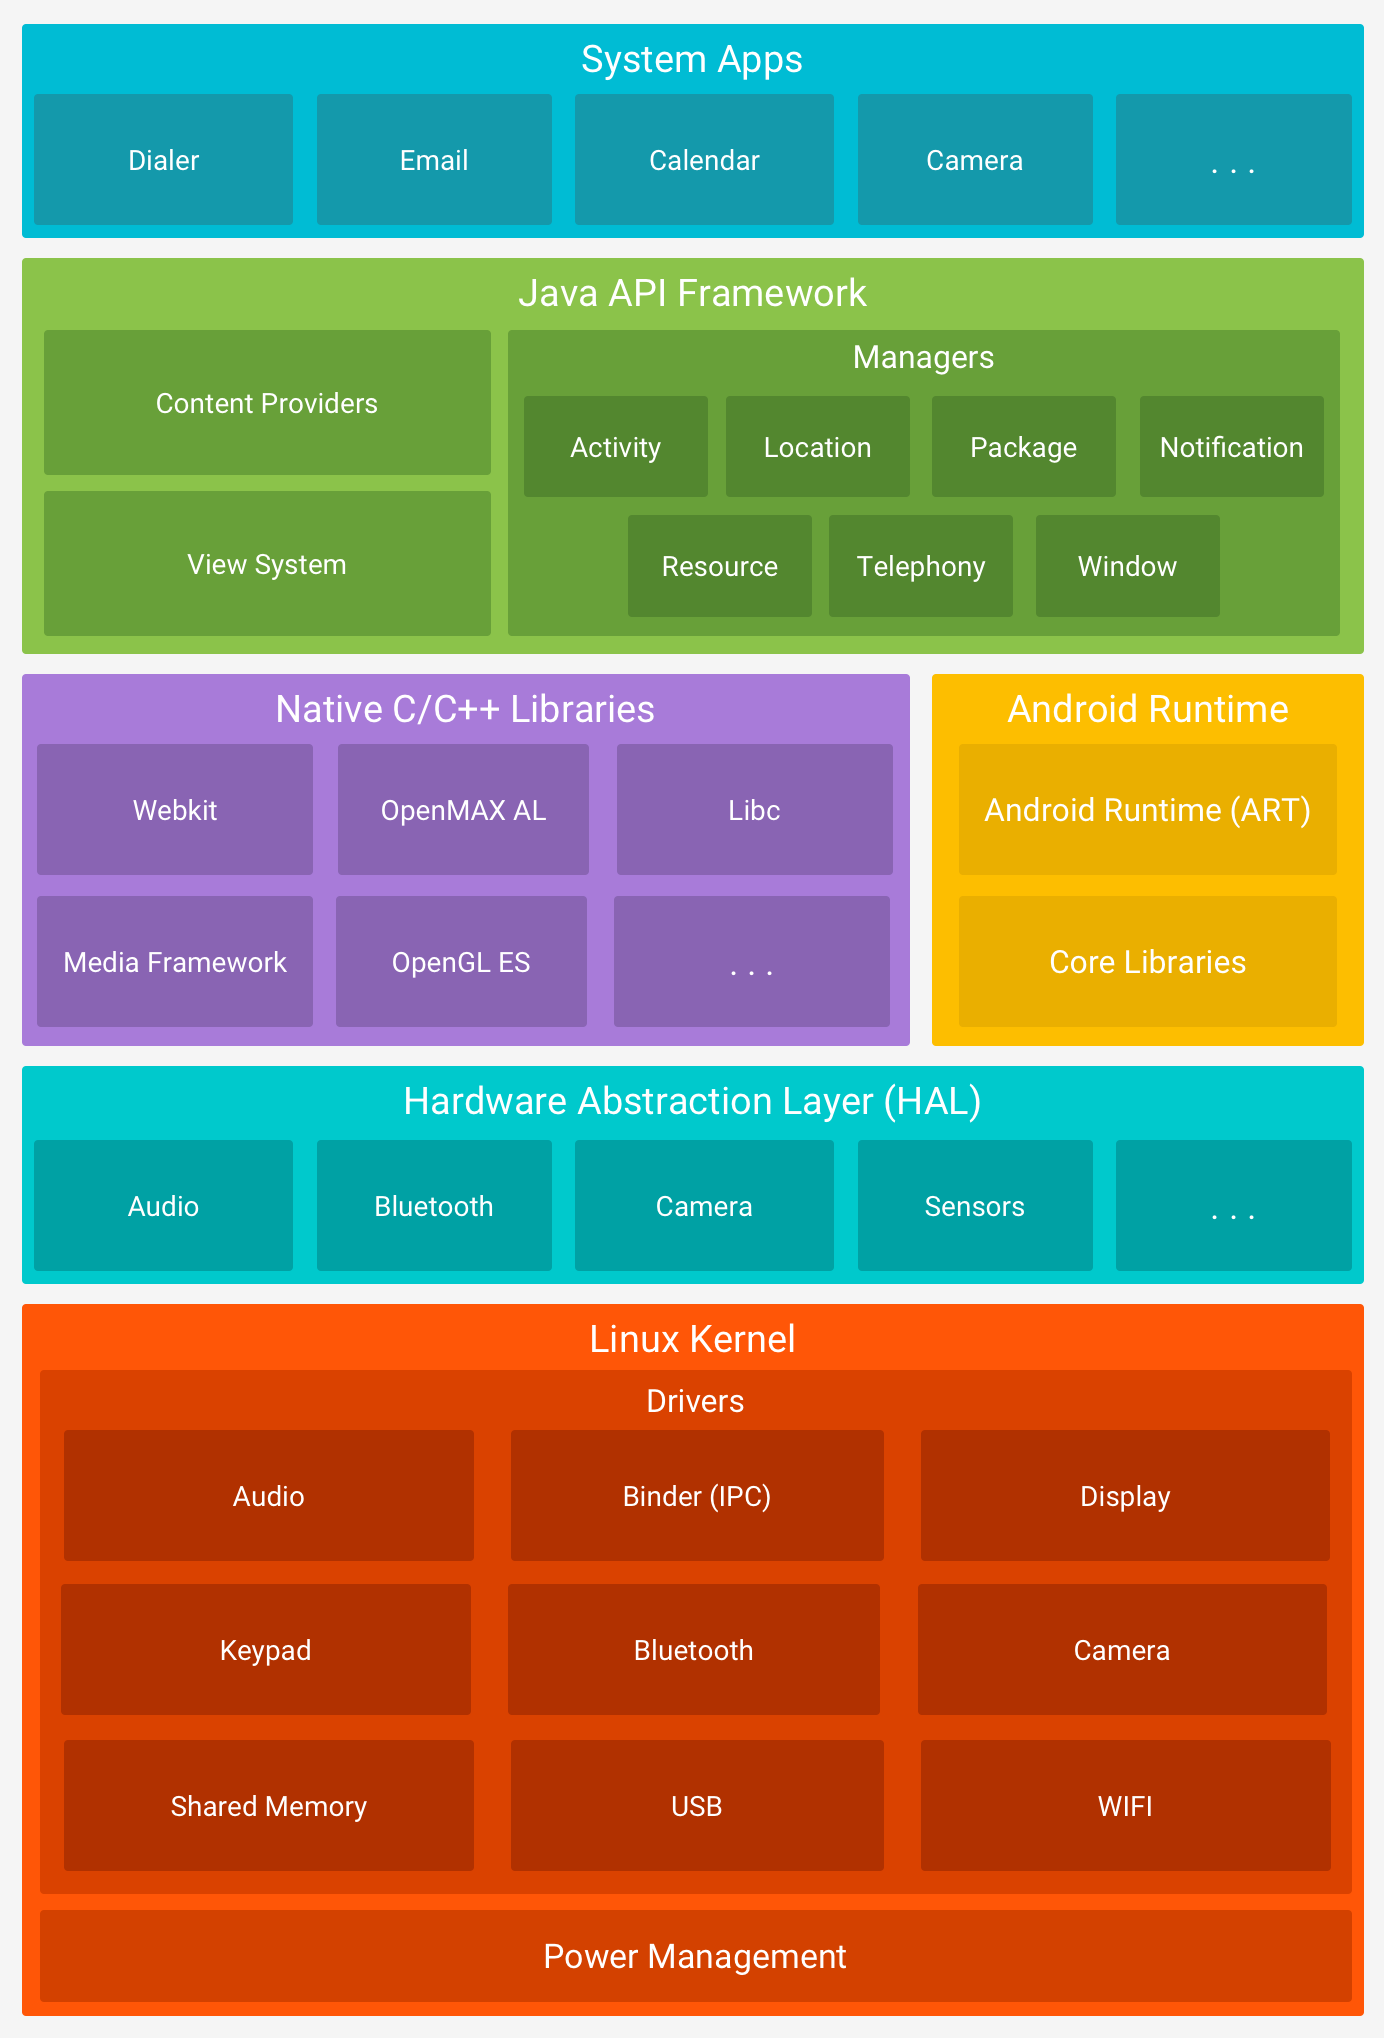
\includegraphics[width=.7\textwidth]{figures/android-stack_2x.png}
    \caption{Android 软件栈示意图}
    \label{fig:android-stack}
\end{figure}

\subsection{AOSP 构建系统历史与现状}

对 AOSP 展开分析的最重要一步是了解 AOSP 的构建过程,而 AOSP 构建系统是解释 AOSP 构建过程的核心关键。本节从 AOSP 构建系统从 GNU Make 到 soong 的演化历史出发,比较了二者在实际应用上的表现并介绍了 soong 中的重要组件与工作方式。

\subsubsection{Android Marshmallow 前:GNU Make}

截至 2015 年上半年,AOSP 所使用的构建系统仍旧依托于 GNU Make——各个模块通过编写各自的 Android.mk 文件,完成对 Android.mk 当前目录下所有源文件的编译以及最终产物的生成。在这一阶段,AOSP 为 GNU Make 提供了统一的编译入口,使用 Makefile 语言的指令将众多仓库下的模块一同构建。由于 GNU Make 的本质是执行给定指令,因此对于使用多种通用编程语言的 AOSP,GNU Make 是一个优秀的顶层构建系统。

然而,随着 AOSP 软件规模的不断增长,GNU Make 逐渐暴露出它的不足之处:

\begin{itemize}
    \item GNU Make 下的 Makefile 文件存在一定的逻辑语句,语法仍较为复杂。Makefile 语法较为灵活,存在诸如分支逻辑、循环逻辑等结构,这为项目开发人员以及软件分析人员带来的较大的困难。
    \item GNU Make 下的 Makefile 需要在每个模块构建之初消除先前模块构建过程中定义的环境变量所带来的影响,进而产生了大量必要且重复的 Makefile 代码。
    \item GNU Make 下的 Makefile 在 AOSP 庞大的系统下,很难在尽量降低对其他模块构建产生影响的同时,对特定模块进行定制化构建工作。
    \item GNU Make 在实际应用过程中,暴露出构建缓慢、难以统一管理等问题。
\end{itemize}

\subsubsection{Android Nought 后:soong / Ninja}

出于对以上问题的考虑,Google 决定将 AOSP Marshmallow 作为最后一个使用 GNU Make 为主要构建系统的大版本,并从 2015 年 1 月起开发适用于 AOSP 的新顶层构建系统——soong。与此同时,Google 采用 Ninja 这一已在 chromium 项目中得到认可的底层构建系统作为代替 GNU Make 构建图生成、构建时资源调度以及提供指令执行环境的工具。

自 Android Nought 开始,AOSP 的构建系统在逐渐从 GNU Make 向 soong / Ninja 过渡。截至目前,AOSP 仍旧存在使用 GNU Make 时期的 Android.mk 文件作为模块构建方式声明的 manifest 文件。

\subsection{soong 构建系统概述}

作为 AOSP 的顶层构建系统,soong 需要负责处理 AOSP 内部的复杂性。为了摒除 AOSP 内多语言项目间构建差异与各模块内与模块间引用带来的影响,soong 需要多个组件来完成整体构建过程。

\subsubsection{Blueprint}

在计划逐步抛弃 GNU Make 后,soong 同样需要一种用于描述 AOSP 中各模块内部与模块间的引用关系的文件协议。通过借鉴 Google 公司开发的另一个构建系统 “Bazel.build” 使用的 manifest 语法,soong 对其进行改造后设计形成了以 “bp” 为文件后缀名的 “Blueprint / Android.bp” 文件,用以替换原本各模块中的 Android.mk 文件。

目前,绝大多数模块使用 Android.bp 文件作为模块构建过程的声明文件(如 frameworks/base)。对 bp 文件格式的解析需要有一个独立的 Blueprint 模块完成,在当前版本的 soong 中,Blueprint 模块完成了对 bp 文件内容语法语义的解析。

相比于在较大程度上依赖于 AOSP 目录结构的 soong 构建系统而言,Blueprint 模块是一个十分独立的部件。这是由于 Blueprint 模块在设计之初,Google 公司希望设计一套能够独立于 AOSP 或 soong 使用的构建过程描述语法,因此在程序设计中,可以将 Blueprint 或 Blueprint 中的部分模块抽出应用到新系统当中。

\subsubsection{Kati}

相较于 soong,Kati 为 AOSP 服务的历史更为悠久。在 Android Marshmallow 前,以 GNU Make 为核心的构建体系已经暴露出构建速度不足的缺陷。Kati 起初担负着加速编译的责任。然而随着 soong 的出现与不断完善,AOSP 已经不需要 Kati 加快构建速度。因此 Kati 仅保留了部分功能(即将 Android.mk 文件中内容转化为符合 ninja 文件协议的约定)。

正如上文所述,截至 Android Tiramisu 版本,AOSP 中仍存在部分模块使用 Android.mk 作为模块构建过程的声明文件(如 development/testrunner)。因此,Kati 模块在当前 soong 系统中依然发挥着巨大的作用。

\subsubsection{Ninja}

Android Nought 后使用已在 chromium 项目中得到认可的 Ninja 作为底层构建工具。

Ninja 将其他构建系统视为 “高级程序设计语言”,同时将自己定位为那些 “高级语言” 对应的 “汇编语言”\cite{NINJABUILD}。也就是说,Ninja 旨在提供一个高效的命令执行环境。任何可用于项目构建的构建系统,都可以将 Ninja 作为构建后端;任何构建系统都可以通过产生内容合乎规范的、以 ninja 为文件后缀的 manifest 文件以借助 Ninja 来加速构建过程。

Ninja 与 GNU Make 类似,不仅是一个构建系统,还定义了用于描述构建过程的文件协议。与 Makefile 相仿,ninja 同样有能力描述有向无环图(DAG)——将文件视作 DAG 中的节点,将输入文件到输出文件的转化过程视作 DAG 中的边。但是,ninja 删除了 Makefile 中的逻辑控制语句,仅仅使用 “输出-输入” 进行描述。

在 soong 运行之初,系统下仅有 soong 系统的源代码,并不能直接使用上述提及的工具。soong 最大的一个特点是允许 “自启动”。在 soong 第一次运行时,系统会自动编译名为 soong\_ui 的二进制文件,该文件作为此后用户使用 soong 其他功能的入口。soong\_ui 的执行也是分阶段的,在初始阶段,soong\_ui 会进行一系列配置,并同时生成名为 Android.bp.list 文件。

此后,soong 进入 minibootstrap 阶段。soong 在本阶段会创建描述构建过程的 manifest 文件并调用 Ninja 开始构建。接下来,soong 进入 bootstrap 阶段,在当前版本 Android Tiramisu 下,soong 并不负责直接构建 AOSP 中的各个模块,而是负责生成 Ninja 所需要的 manifest 文件——build.ninja。因此,与其说 soong 是一个构建系统,不如说 soong 是一个 manifest 文件转换工具。

\begin{figure}[h]
    \centering
    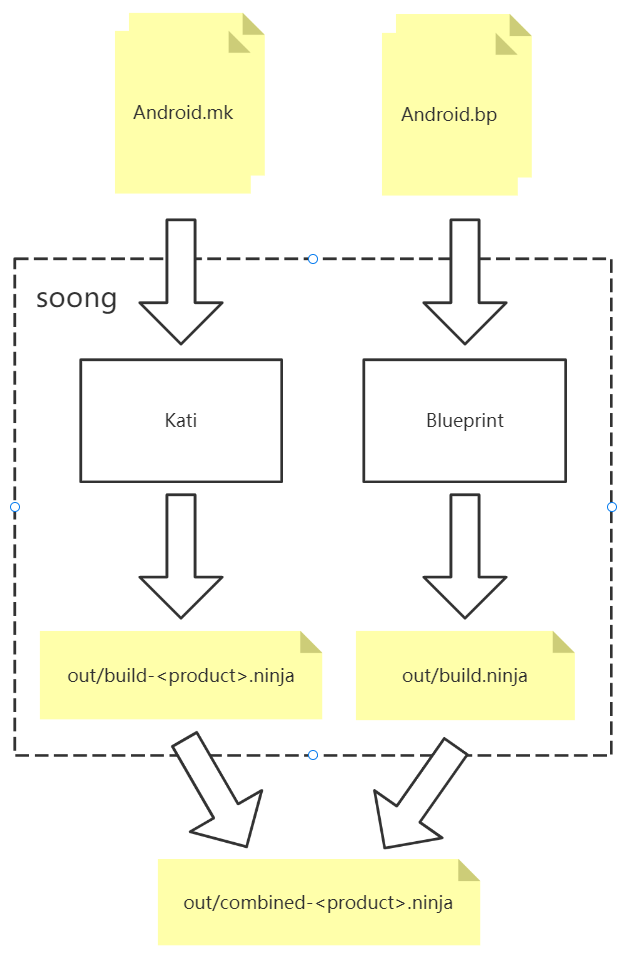
\includegraphics[width=.4\textwidth]{figures/soong-arch.png}
    \caption{soong 构建系统工作示意图}
    \label{fig:soong-architecture}
\end{figure}

对于当前版本的 soong 构建系统而言,其在构建方面主要由 Blueprint 与 Kati 两个转换工具构成——前者负责使用 soong\_ui 生成的 Android.bp.list 文件收集各模块下的 Android.bp 文件并生成 build.ninja,后者负责收集各模块下仍未调整至 Android.bp 文件的 Android.mk 文件并生成 build-<product>.ninja。这两份 ninja 文件是 AOSP 构建对应目标的清单文件,其中详细叙述了该目标可能需要的所有构建过程。

此后,soong 会将二者使用 subninja 语法链接到名为 combined-<product>.ninja 文件中,并将该文件输入至 Ninja,作为 Ninja 开展 AOSP 构建过程的输入之一。在 soong 运行的最后阶段,soong 会创建 Ninja 进程,使用先前生成的 combined-<product>.ninja 文件开始 AOSP 的构建。soong 的整体架构如图 \ref{fig:soong-architecture} 所示。

\subsection{对 AOSP 展开分析的重要性}

在 Google 公司的主导下,AOSP 的维护行为十分频繁,对主要核心仓库的代码变动较大。根据 Google 的 Android Git repositories 中记载,仅 frameworks/base 仓库在 android-12.0.0\_r1 与 android-11.0.0\_r35 两个版本之间就有 151234 个提交记录,其中含有 21611 个非合并提交。其中,存在部分提交涉及数十个文件的核心代码变更。

当前活跃于市场的大多数 Android 手机的核心系统都是基于 AOSP 进一步开发。然而,在 Google 公司发布 AOSP 新版本时,各大公司均需要合入 Google AOSP 的软件变更,这为基于 AOSP 的移动系统研发部门带来了相当大的挑战。

\subsection{分析 AOSP 过程中遭遇的困难}

AOSP 作为 Android 系统的核心组成部分,是一个复杂的整体概念。对其直接展开分析是极其困难的。在对 AOSP 的整体架构进行学习之后,我主要总结出以下三点困难。这三点困难使得对 AOSP 的分析相对于其他软件项目(如 Java Web 项目、Android 应用等)更为复杂。

\begin{itemize}
    \item 独特的构建系统:Android Marshmallow 后,Google 公司选用 soong 作为 AOSP 的顶层构建系统来代替 GNU Make,并使用 ninja 作为底层构建系统加速构建过程。非泛用的构建系统为基于 AOSP 的变更分析带来了设计上的特殊性。
    \item 丰富的编程语言:AOSP 中掺杂了多种通用编程语言,包括但不限于 C,C++,Java,Kotlin,Go,Python 等。编程语言的不统一为基于源代码的分析带来了相当的复杂性。以编程语言多样性相呼应的,是项目结构的多样性。AOSP 由成千上万个不同的项目共同构成,不同的语言所使用的项目结构规范也都不相同,这使得目前许多软件分析工具无法胜任全部工作,必须针对具体情况展开具体分析。
    \item 庞大的系统架构:以 platform/frameworks 为例,其由 67 个仓库组成,共有 5804 个模块,而 AOSP 共拥有数千个代码仓库。与代码仓库数目众多相匹配的,是 AOSP 高度活跃的社区。在 Google 的带领下,大版本间代码变动大成为了 AOSP 的特性之一。
\end{itemize}

\newpage
\section{软件变更获取}\label{software-diff-extract}

进行软件变更分析首先需要获取软件变更,一般情况下,变更获取算法可基于纯文本或基于树结构进行分析。在对 AOSP 进行分析的场景下,借助 git 这一版本控制管理中的对象文件可以更好地获取变更信息——git 可获取的变更信息大致被分为两类,分别是变更文件元数据信息以及具体文本差异。本节讨论了两类方法在该场景下的优劣,并给出了适当的变更获取算法。

\subsection{基于纯文本的变更获取算法}

获取软件变更的最简便方法是使用基于纯文本的变更获取算法。

Webb Miller 等人提出了一段基于文本的文件对比程序\cite{SPAE-1985-AFileComparisonProgram}。文章中给出了简洁的文件对比程序项目源码。Muhammad Asaduzzaman 等人提出了一种基于文本的语言无关文本差异获取算法\cite{ICSM-2013-AsaduzzamanRSP}。算法通过建立 “候选列表” 猜测源文件到目标文件的可能映射,使用摘要算法确定对应关系。因此,分别获取两个版本中的所有文件并进行比较是一种获取变更差异的可行方案。

由于 AOSP 中所有仓库都使用 git 作为版本控制系统,而 git 中使用二进制对象存储了相邻两个版本之间的软件变更情况(文件内容增加与删除情况),且 git 中实现过 Myers、Minimal、Patience 以及 Histogram 四种文本差异算法\cite{Nugroho_2019},所以任意两个版本之间的软件变更都可以通过 git 获取。但需要注意的是,git 作为通用版本控制系统,其中用于得出两版本间差异的算法是与语言无关的文本差异算法,不存在对于特定文本文件类型优化的情况。也就是说,基于 git 内部数据结构实现的变更获取算法必定是基于纯文本的。然而,上文提及的纯文本变更获取算法存在着下述问题:

\begin{itemize}
    \item 基于纯文本的变更获取算法很难进行空间与时间复杂度的权衡。
    \item 现有基于纯文本的变更获取算法在程序设计方面较为简洁,很难提升程序的可扩展性。
    \item 基于纯文本的变更获取算法忽视了源文件中的代码结构。
\end{itemize}

基于纯文本的变更差异分析仅仅能够获取方法名,但对于方法的形参获取存在一定的困难。这种困难主要是程序设计上的。因此放弃 AST 选用纯文本意味着放弃了具有足够表达能力的工具,也同时意味着获取方法形参类型代码片段必定具备相当的复杂性。

\subsection{基于树的变更获取算法}

软件分析并不需要将项目中所有文件都纳入分析范围。一个项目中可能存在相当大部分的文件与项目核心功能无关。这些无关文件的修改并不会对项目核心功能造成影响。更进一步地,仅仅考虑核心代码文件而忽视诸如文本文件、配置文件、测试文件等无关文件,可能会在降低分析任务量、提高分析速度的同时,不丧失对项目核心功能变更的把控。相较于基于纯文本的变更获取算法,基于树的变更获取算法不再忽视源文件中的结构,可以获取更细粒度的变更信息。

Jean-Remy Falleri 等人提出了一种细粒度的源代码差异分析算法,并实现了名为 gumTree 的变更获取工具\cite{DBLP:conf/kbse/FalleriMBMM14}。该算法作为一种语言相关的算法,不再以 “行” 作为最小单元,而是以抽象语法树为基础,以抽象语法树叶子节点作为最小单元。但该工具的实现并没有在其建立的树结构与抽象语法树之间建立联系,这使得该工具专注于变更节点,而难以获取变更节点的父子节点信息。

\subsection{变更信息种类}

变更信息种类会受到变更获取算法所属种类的影响。基于文本的变更获取算法通常以 “行” 为构成文件的基本单元,所以此类算法仅可以给出源文件到目标文件的 “新增行” 与 “删减行” 的列表。相较于此,基于树的变更获取算法可以通过设置 “抽象语法树节点”、“表达式”、“语句” 等不同粒度来满足分析需要。

在本文所设计的软件变更分析系统中,我综合使用了两类变更获取算法——使用基于文本的变更获取算法,如图\ref{fig:git-alg}所示分析给定软件在两个版本之间存在变更的文件;使用基于树的变更获取算法\ref{alg:get-method-name},获得给定软件在两个版本之间遭到修改的方法名。

\begin{figure}
    \centering
    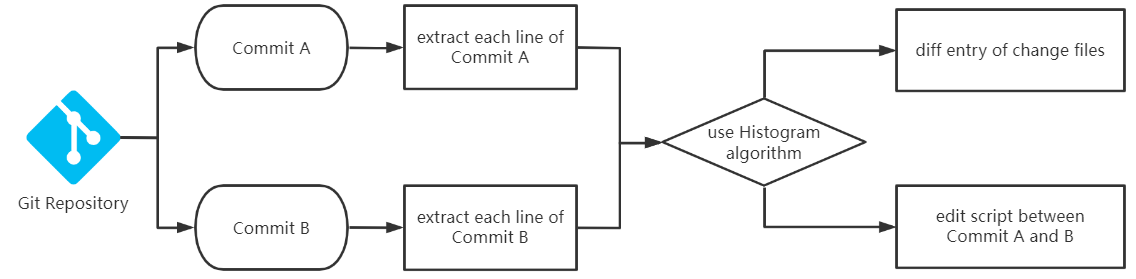
\includegraphics[width=.8\textwidth]{figures/git-alg.png}
    \caption{使用 git 获取两版本间变更文件}
    \label{fig:git-alg}
\end{figure}

\renewcommand{\thealgorithm}{1}
    \begin{algorithm}
        \caption{方法名获取算法}
        \begin{algorithmic}[1]
            \Require 差异文件入口到文本差异的映射 $M$
            \Ensure 差异文件信息 $Info$
            \State initialize $l$ as a list
            \For{$(entry, script) \to M$}
                \State $tree \Leftarrow entry.node$
                \If{tree's ancestor exists "MethodDeclaration"}
                    \State $l \Leftarrow tree$
                \EndIf
            \EndFor
            \For{$node \in l$}
                \State get $methodName$ by node's ancestor
                \State $Info \Leftarrow methodName$
            \EndFor
            \State \Return $Info$
        \end{algorithmic}
        \label{alg:get-method-name}
    \end{algorithm}
\newpage
\section{模块间分析}\label{intermodule-analysis}

模块间分析是本文所设计的软件变更分析系统中最为重要的部分。AOSP 由若干仓库组成,各仓库又由若干模块组成,然而各仓库与模块并非完全封闭的。在构建时,某仓库下的模块可能会使用其他仓库下的另一模块,这导致单模块变动可能产生难以想象的影响。因此,对 AOSP 进行模块间分析是极其重要的。本节从 soong 的模块概念入手,扩展了有向图概念,提出了基于 AOSP 完全构建过程的模块间分析算法。

\subsection{soong 的模块概念}

soong 作为 Android Tiramisu 使用的顶层构建系统,继承了 Android Nought 以 GNU Make 为主导的构建系统下模块的概念,如图\ref{fig:aosp-3-layer}所示使用 “仓库-模块-文件” 三层为庞大的 AOSP 分级。

\begin{itemize}
    \item Google 使用 git 作为 AOSP 的版本控制系统,进而使得仓库成为 AOSP 最上层结构单元。
    \item soong 使用 Android.bp 对 AOSP 进行下一层分级。本文所设计的软件变更分析系统将 Android.bp 所在路径下的所有文件视为同一模块。
    \item 文件既可以是用于产生编译产物的输入文件,也可以是单次构建过程的输出文件。文件是 AOSP 构建系统视角下的最基本单元。
\end{itemize}

\begin{figure}
    \centering
    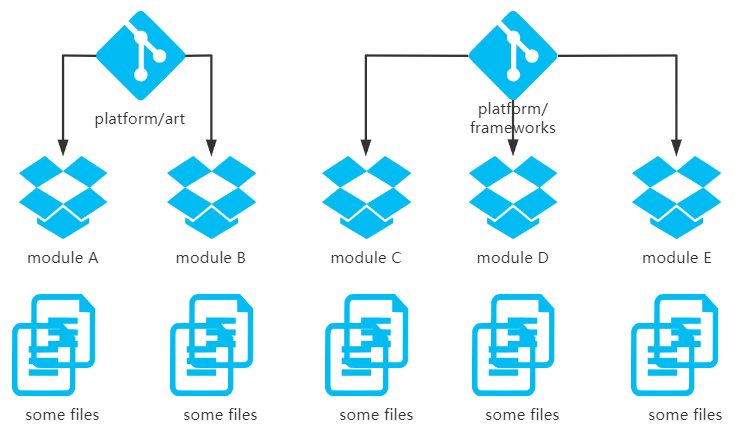
\includegraphics[width=.8\textwidth]{figures/3-layer.png}
    \caption{AOSP 三层架构}
    \label{fig:aosp-3-layer}
\end{figure}

\subsection{有向无环图}

\begin{dfn}
    给定一个有序的二元组 $<V, E>$,其中 $V$ 是一个被称作 “顶点集” 的非空有穷集。$\forall v \in V$, $v$ 被称作 “顶点”。当 $E$ 是笛卡尔积 $V \times V$ 的有穷多重子集时,$\forall e \in E$,$e$ 被称作 "有向边"。\cite{DISCRETEMATH}
\end{dfn}

\begin{dfn}
    设 $D = <V, E>$ 为有向图,$e_k = <v_i, v_j> \in E$,称 $v_i, v_j$ 为 $e_k$ 的端点,$v_i$ 为 $e_k$ 的始点,$v_j$ 为 $e_k$ 的终点。\cite{DISCRETEMATH}
\end{dfn}

\begin{dfn}
    设 $D = <V, E>$ 为有向图,$\forall v \in V$,称 $v$ 作为边的始点的次数为 $v$ 的出度,记作 $d^+(v)$,称 $v$ 作为边的终点的次数为 $v$ 的入度,记作 $d^-(v)$。
\end{dfn}

根据定义,图中有两类基本元素:节点可以用于抽象现实生活中的具体事物;边可用于抽象节点间的关系。有向图中通常使用有向边来表示节点间的偏序关系,以 $v_i$ 为始点,$v_j$ 为终点的边 $e$ 表示 $v_i \prec v_j$。而通过基于图的拓扑排序算法,可以得到有向图中一系列节点间的偏序关系集合。

\begin{dfn}
    给定一个有向图 $D = <V, E>$,其拓扑排序(见算法 \ref{alg:topology-sort})是它的顶点的线性排序。若图中存在两顶点 $v_i, v_j \in V$,则存在一条有向边 $e \in E$,且 $e$ 以 $v_i$ 为始点,$v_j$ 为终点,则记该有向边为 $e_{u v}$。在拓扑排序中,$i$ 在 $j$ 之前。
\end{dfn}

根据拓扑排序算法的定义,该算法包含了图中节点关系问题的解决方案。拓扑排序可被应用在调度任务上——图中节点被用于表示任务、图中有向边被用于表示任务间依赖关系。如果任务 $i$ 必须在任务 $j$ 开始之前完成,则存在一条从 $v_i$ 到 $v_j$ 的边。

对于任务调度问题而言,单一任务在调度全过程中只出现一次。也就是说,给定一个任务 $i$,其入度 $d^+(v_i) \le 1$,但不对其出度 $d^-(v_i)$ 做限制。由此可得,所有入度为 0 的节点 ${v'}_k \in V, (d^+(v_k) = 0)$ 是可以立即执行的任务。

\begin{dfn}
    设 $D = <V, E>$ 为有向图,$D$ 中顶点与边的交替序列 $\varGamma = v_{i_0} e_{i_0 i_1} v_{i_i} ... v_{i_{k-1}} e_{i_{k-1} i_k} v_{i_k}$ 称作节点 $v_{i_0}$ 到节点 $v_{i_k}$ 的通路。若 $v_{i_0} = v_{i_k}$,则称其为回路。
\end{dfn}

此外,为满足单一任务仅仅被执行一次,图中任意一个节点 $v_k \in V$,都不应存在一条回路。满足以上性质的图被称作有向无环图(如图\ref{fig:dag}所示)。

\begin{figure}
    \centering
    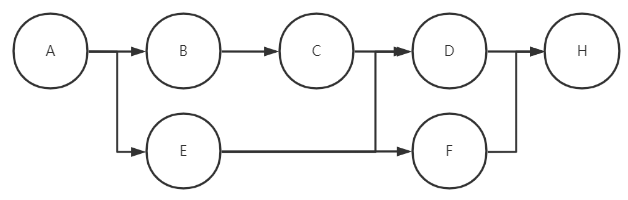
\includegraphics[width=.7\textwidth]{figures/dag.png}
    \caption{有向无环图示例}
    \label{fig:dag}
\end{figure}

\renewcommand{\thealgorithm}{2}
    \begin{algorithm}
        \caption{有向图拓扑排序算法}
        \begin{algorithmic}[1]
            \Require 输入有向图 D = <V, E>
            \Ensure 有向图是否有环
            \State initialize $q$ as a queue // 初始化队列
            \For{$i = 1 \to n$}
                \If{$D.E[i].indegree = 0$}
                    \State $q \Leftarrow E[i]$
                \EndIf
            \EndFor
            \While{$q$ is not empty}
                \State $temp \Leftarrow$ first element in $q$
                \For{$i = 1 \to n$}
                    \If{$(V_{temp} \to V_{i}) \in D.E$}
                        \State $D.E[i].indegree \Leftarrow D.E[i].indegree - 1$
                        \If{$D.E[i].indegree = 0$}
                            $q \Leftarrow D.E[i]$
                        \EndIf
                    \EndIf
                \EndFor
            \EndWhile
            \State \Return $C_1, C_2$ //输出结果
        \end{algorithmic}
        \label{alg:topology-sort}
    \end{algorithm}

结合有向图拓扑排序算法,可易得引理\ref{lem:dag}。

\begin{lem}
    一个有向图 $G = <V, E>$ 是无环的当且仅当对其进行的深度优先搜索不产生后向边。\cite{DBLP:books/daglib/0023376}
    \label{lem:dag}
\end{lem}

然而不足的是,拓扑排序受到有向图定义的限制,一条边仅能够连接始点与终点两个节点。这一缺陷降低了简单有向图对实际问题的抽象能力,下一小节将拓展现有有向图概念,使之具备描述构建系统中构建过程的能力。

\subsection{完全构建过程}

对于一个构建系统而言,其用于描述完全构建过程的 manifest 中定义了一系列独立构建过程的集合 $B$。对于单一过程 $b \in B$,其具备输入文件 $f_{in}$ 以及输出文件 $f_{out}$,可将该过程记为 $b_{<f_{in}, f_{out}>}$。若将所有输入输出文件的并集 $\bigcup_{b_{<f_{in}, f_{out}>} \in B} (f_{in} + f_{out})$ 记作 $F$,则 manifest 中定义的完全构建过程可被表示为 $P = <F, B>$。

由有向图概念可知,完全构建过程 $P$ 是一种扩展了 “边” 概念的有向图。在有向图中,$E$ 是顶点集 $V$ 的笛卡儿积 $V \times V$ 的有穷多重子集。而在完全构建过程中,$B$ 是文件集合 $F$ 非空子集 $f \subseteq F\ and\ f \neq \emptyset$ 的笛卡儿积 $f \times f$ 的有穷多重子集。后称满足上述性质的数据结构为 “扩展有向图”(如图\ref{fig:build-process}所示)。

\begin{figure}
    \centering
    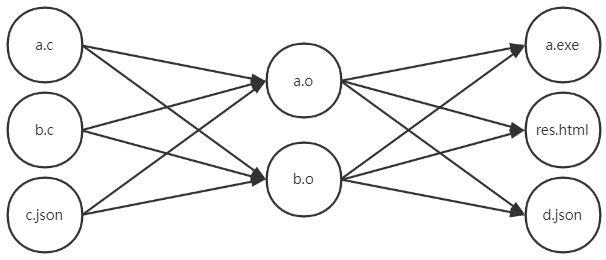
\includegraphics[width=.7\textwidth]{figures/build-process.png}
    \caption{构建过程示例}
    \label{fig:build-process}
\end{figure}

基于对项目构建的概念理解,完全项目构建具有以下特性。

\begin{enumerate}
    \item 构建过程涉及的文件数目是有限的。
    \item 构建过程是有限的。
    \item 正常的构建过程是可终止的。
    \item 出现在构建过程中的文件,其生成方式不超过一种,即:某文件不可能同时被两种方法生成。
\end{enumerate}

由有向图概念,同理可得完全构建过程 $P = <F, B>$ 的对应概念。

\begin{lem}
    给定一个完全构建过程 $P = <F, B>$,其中 $V$ 与 $B$ 是有限集。
\end{lem}   

\begin{lem}
    给定一个完全构建过程 $P = <F, B>$,定义对其中单一构建过程之间的 “拓扑排序” 为完全构建过程 $P$ 中所涉及文件集合 $F$ 的线性排序。规则为:若图中存在两顶点 $f_i, f_j \subseteq F$,则存在一条有向边 $b \in B$,且 $b$ 以 $f_i$ 为始点,$f_j$ 为终点,则记该有向边为 $b_{<f_i, f_j>}$。在拓扑排序中,$f_i$ 中所有文件 $f' \in f_i$ 在 $f_j$ 中所有文件 $f'' \in f_j$ 之前。
\end{lem}

由于对项目构建过程是可自行终止的,所以对完全构建过程 $P = <F, B>$ 进行拓扑排序可根据有向图拓扑排序算法扩展为算法 \ref{alg:total-build-topology-sort}。

\renewcommand{\thealgorithm}{3}
    \begin{algorithm}
        \caption{完全构建过程的拓扑排序算法}
        \begin{algorithmic}[1]
            \Require 输入完全构建过程 P = <F, B>
            \Ensure 完全构建过程是否有环
            \State initialize $q$ as a queue // 初始化文件队列
            \For{$i = 1 \to n$}
                \If{$D.E[i].indegree = 0$}
                    \State $q \Leftarrow E[i]$ // 获取所有源文件
                \EndIf
            \EndFor
            \While{$q$ is not empty}
                \State $temp \Leftarrow$ first element in $q$
                \For{$b \in temp.outEdges$}
                    \For{$f \in b.outputFiles$}
                        \If{$f \in q$}
                            \State \Return false
                        \EndIf
                        \State $q \Leftarrow f$                         
                    \EndFor
                \EndFor
            \EndWhile
            \State \Return true
        \end{algorithmic}
        \label{alg:total-build-topology-sort}
    \end{algorithm}

\subsection{Ninja 中对构建过程的描述}

为提供一个高效的指令执行环境,Ninja 定义了一套不同于 Makefile 的 manifest 语法(由于 Ninja 的 manifest 文件以 “ninja” 作为后缀,此后使用 ninja 代指这套 manifest 语法)。

相较于 Makefile,ninja 去除了诸如 “分支语句”、“过程定义”、“变量覆写” 等复杂语法,极大地降低了 Ninja 构建系统在运行时所需工作。ninja 专注于简洁地叙述构建过程,其语法能够最为简单地描述构建过程。

ninja 使用 “rule” (后文称为 “规则”)定义有向无环图中的边类型。在规则中,需要定义具体执行的语句,同时放置输入输出参数到恰当位置中。在规则被调用时,输入文件会被传入,同时生成符合要求的输出文件。除执行语句外,在规则语法中还可以定义最大线程数等参数进行优化。ninja 中的规则支持多输入文件到多输出文件的映射,且输入文件按照是否直接出现在执行语句中被分为 “直接依赖”、“间接依赖” 以及 “order only 依赖” 三种。ninja 使用 “build” (后文称为 “构建”)声明并实例化有向无环图中的边。ninja 格式的文件中定义了一系列构建(以 soong 构建系统产物之一 build.ninja 为例,其中使用了 90\% 以上文本描述构建)。构建是规则的实例化表现形式,其需要指定所使用的规则名,并给出规则内语句执行时需要的具体输入文件。

\subsection{模块间分析算法}

作为本文所设计软件变更分析系统的一部分,模块间分析需要根据发生变更的文件得出该变更可能影响的所有文件。

在有向图中,根据给定数量的节点搜索可达路径上所有节点的问题被称作 “多源可达问题”。然而,模块间分析并不完全等价于 “多源可达问题”。基于 Ninja 构建系统定义的完整构建过程 $P = <F, B>$ 以及实际构建过程中模块间的影响,模块间影响可分为以下两种情况。

\begin{enumerate}
    \item 文件 $a$ 改变,$\exists\ b_{<f_{in}, f_{out}>} \in B$,且文件 $a \in f_{in}$,$f_{out}$ 中所有文件受到直接影响,而 $f_{out}$ 可能被认定属于其他模块。如图\ref{fig:inter-module}中 a.2 对 a.3 的影响。
    \item 文件 $a$ 改变,$\exists\ b_{<f_{in}, f_{out}>} \in B$,且文件 $a \in f_{in}$,$f_{in}$ 中所有除 $a$ 之外的文件都可能因 $a$ 的改变而受到间接影响,而 $f_{in}$ 中其他文件可能来自于其他模块。如图\ref{fig:inter-module}中 a.2 对 sub.3 与 sub.4 的影响。
\end{enumerate}

\begin{figure}
    \centering
    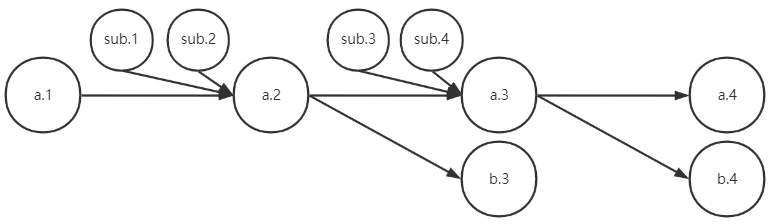
\includegraphics[width=.8\textwidth]{figures/inter-module.png}
    \caption{模块间影响示意图}
    \label{fig:inter-module}
\end{figure}

在传统有向图中,“多源可达问题” 可使用图搜索算法解决。而在扩展有向图中,上述结论仍旧成立。对于深度优先搜索算法与广度优先搜索算法,在解决该问题时,存在以下可供权衡的观点。

\begin{itemize}
    \item 深度优先搜索是求解 “多源可达问题” 的最通用算法。然而在构建问题背景下,很难通过深度优先算法获得必要的构建次序信息。
    \item 广度优先搜索通过维护文件队列搜索扩展有向图。然而 AOSP 的体量庞大,需要大量单元表示文件状态。
\end{itemize}

为获取有关构建过程的更多信息,本文所设计的软件变更分析系统采用广度优先搜索,如算法\ref{alg:intermodule-analysis}所示。综上所述,在扩展有向图 $P = <F, B>$ 中搜索可能受影响文件的本质仍是图可达性问题,该问题仍可在 $O(F + B)$ 中解决。\cite{GRAPHREACHABILITY}

\renewcommand{\thealgorithm}{4}
    \begin{algorithm}
        \caption{基于 Ninja 的过程间分析算法}
        \begin{algorithmic}[1]
            \Require 输入完全构建过程 $P = <F, B>$
            \Require 输入被修改的文件集合 $F_{in}$
            \Ensure 被直接影响的文件集合 $F_{direct}$
            \Ensure 被间接影响的文件集合 $F_{indirect}$
            \State initialize $q$ as a queue // 初始化文件队列
            \For{$f_{in} \in F_{in}$}
                \State $q \Leftarrow f_{in}$
                \State $F_{direct} \Leftarrow f_{in}$
            \EndFor
            \While{$q$ is not empty}
                \State $temp \Leftarrow$ first element in $q$
                \State $outputFiles \Leftarrow$ get all output files by $temp$
                \For{$f \in outputFiles$}
                    \If{$f \notin F_{direct}$}
                        \State $q \Leftarrow f$
                        \State $F_{direct} \Leftarrow f$
                    \EndIf
                \EndFor
            \EndWhile
            \For{$fd \in F_{direct}$}
                \State $inputFiles \Leftarrow$ get all input files by $fd$
                \For{$f \in inputFiles$}
                    \If{$f \notin F_{direct}$}
                        \State $F_{indirect} \Leftarrow f$
                    \EndIf
                \EndFor
            \EndFor
            \State \Return $F_{direct}, F_{indirect}$
        \end{algorithmic}
        \label{alg:intermodule-analysis}
    \end{algorithm}

\newpage
\section{模块内分析}\label{intramodule-analysis}

模块内分析是本文所设计的软件变更分析系统中的重要模块。在已知某文件存在变更时,可通过 Ninja 的构建过程描述文件确定中间产物,进而完成对模块内的分析。本节讨论了 Java 语言在变更系统中的应用,选用调用图作为模块内分析工具,并比较了三种可生成调用图的开源工具。

\subsection{模块内分析的困难}

相较于基于 soong 构建系统与 Ninja 底层构建系统的模块间分析,对 AOSP 展开模块内分析拥有更大的复杂性。如第\ref{aosp-build-system}节所述,soong 为了解耦构建过程,借鉴了跨语言构建系统 “Bazel.build” 的语法定义了 Android.bp 文件中使用的 Blueprint 语法,并用 Blueprint 组件将 Android.bp 文件中定义的模块构建方法转化为对应的 ninja 构建规则。也就是说,soong 处理了 AOSP 中多种通用编程语言的复杂性。

然而,soong 仅仅用于构建领域,进行模块内分析无法借助 soong 的组件降低语言复杂性。因此,为每种语言分别撰写分析程序成为 AOSP 模块内分析的唯一途径。尽管不同种语言间分析程序并无差异,但囿于工作量庞大,本文所设计的软件变更分析系统仅考虑 Java 语言在 AOSP 中的应用,并仅考虑 platform/frameworks 下的 67 个仓库,共计 5804 个模块。

\subsection{调用图}

在程序分析当中,存在需要对控制流进行分析的情况。调用图用于描述过程间控制流与数据流,是一种可以保守地逼近程序的过程间控制流的方法。调用图中存储了给定程序中被调用的所有函数以及每个被调用函数的调用点\cite{MoellerS20}。静态调用图往往过分估计调用图中边的数量,这是因为在 OOP 语言中,一个方法的调用与运行时的接收器类型有关\cite{JSP19}。OOP 语言会因 “继承” 特性导致子类可以继承父类中定义的方法。而由于 “继承” 特性的存在,父类中可以通过定义抽象方法交由子类具体实现,而实现 OOP 语言中的 “多态” 特性。由于这种特性在作用时,对于某一个方法无法根据程序代码信息 “静态” 地分析出接收器类型。在经典的程序分析方法中,在 “准确性” 与 “完整性” 两方面的权衡中一般选择后者。这使得静态代码分析中将抽象方法的调用视作以该父类所有子类类型为接收器类型,以各子类中具体实现的方法为被调用方法的调用。因此,其可能包含过量的调用边,但绝不会遗漏。

Java 中的方法调用主要有三类,分别是 static call、special call 和 virtual call。其中 static call 被用于静态方法,virtual call 被用于类构造函数、私有方法、父类中存在并继承至该类的方法。对于大部分 OOP 语言,此二者在编译时均可确定被调用方法的方法签名,即仅有唯一一种方法可能被调用。而 virtual call 包含了其余所有方法调用情况,包括上述 “多态” 特性下的方法调用。因此,virtual call 在静态分析时的被调用方法数量存在大于 1 个的可能,即只有在运行时才能确定 virtual call 方法的接收器类型,进而才能确定方法签名(由方法所在类、方法名、方法返回类型、方法传入参数类型列表构成)。

\subsection{调用图构建算法}

调用图是进行过程间分析的基础。如上所述,在 Java 中的主要方法调用共有三类,而对应到 JVM 指令则有五种——对应 static call 的 invokestatic,对应 special call 的 invokespecial,对应 virtual call 的 invokeinterface 与 invokevirtual。对于 virtual call,由于其只有在具体执行时才可确定真正的接收器对象类型,而方法调用图需要在静态代码的基础上生成,因此需要有一种算法允许代码在非运行情况下找到最可能的接收器对象类型。也就是说,构建调用图的关键在于确定 virtual call 的方法签名。

在程序分析理论的发展过程中,诸如 CHA、VTA、RTA、k-CFA 等调用图生成算法被相继提出。在我所调研的开源调用图构建工具中,CHA 与 k-CFA 两种算法分别由于效率与准确性出众而被采用。

\subsubsection{CHA 算法 (Class Hierarchy Analysis)}

CHA 算法的本质正如其名,是通过查找类的继承关系(即 “边缘”),获得所有可能的接收器类型。

假定需要求解的方法签名为 $S$,根据上文所述,其可被表示为 $S: <OT: RT MN(ArgT...)>$,其中 $OT$ 为接收器对象的类型,$RT$ 为该方法的返回值类型,$MN$ 为该方法的方法名,$ArgT$ 为该方法的传入参数类型列表。

定义 $Dispatch$ 如算法 \ref{alg:dispatch-algorithm} 所示。

\renewcommand{\thealgorithm}{5}
    \begin{algorithm}
        \caption{方法派发 Dispatch 算法}
        \begin{algorithmic}[1]
            \Require 输入接收器对象类型 $r$
            \Require 输入方法签名 $s$
            \Ensure 输出等价的方法签名 $s'$
            \State $MethodList \Leftarrow c.getMethods$
            \For{$m \in MethodList$}
                \If{$m$ is not an abstract method and $m.name == s.name$}
                    \State \Return $m$
                \EndIf
            \EndFor
            \State $super \Leftarrow r.superclass$
            \State \Return $Dispatch(super, s)$
        \end{algorithmic}
        \label{alg:dispatch-algorithm}
    \end{algorithm}

在 OOP 语言中,时常将子类对象赋值给父类类型,期望后续通过操作父类类型来使用子类中覆写的方法。“多态” 使得用户看似在使用父类对象,实则是在使用子类对象。CHA 算法选择忽略 “多态” 带来的不确定性,将一切方法的接收器类型视作该方法的 “假设调用类型”——具体而言,是将每一个可能被赋给该类型的其余类型纳入考虑范围,如算法 \ref{alg:CHA-algorithm} 所示。在 Soot 中,构造调用图使用 CHA 算法。

\renewcommand{\thealgorithm}{6}
    \begin{algorithm}
        \caption{CHA 算法}
        \begin{algorithmic}[1]
            \Require 调用点方法签名 $s$
            \Ensure 实际方法签名的所有可能 $set$
            \If{$m$ use invokestatic}
                \State \Return $\{s\}$
            \ElsIf{$m$ use invokespecial}
                \State $RT \Leftarrow s.RT$
                \State \Return $\{Dispatch(RT, s)\}$
            \Else
                \State initialize $set$ as empty set
                \State $RT \Leftarrow s.RT$
                \For{$class \in$ \{$RT$ and subclasses of $RT$\}}
                    \State push $Dispatch(class, s)$ in $set$
                \EndFor
                \State \Return $set$
            \EndIf
        \end{algorithmic}
        \label{alg:CHA-algorithm}
    \end{algorithm}

\subsubsection{k-CFA 算法 (k-Control Flow Analysis)}

控制流算法是静态程序分析中用于确定程序内控制流图的技术。由于该算法不再停留在类与方法级别而是进入程序内分析,因此得到的结果更为精确。k-CFA 是一类算法的统称,其含义为:针对某特定过程,根据所有可能可达此过程的 k 阶调用路径进行程序分析\cite{FLOWSENSITIVECONTROLFLOWANALYSIS}。然而,在调用图生成过程中,并不需要这样复杂的上下文。

除开利用类 “边缘” 信息,构建调用图的另一种方法是模拟堆结构。在静态分析中,堆结构通常用来描述对象分配情况。为了描述堆结构,可能需要找出被实例化过的对象类型、程序中创建对象的位置以及程序中可能使用到的所有对象。0-CFA、ZeroOneCFA 以及 ZeroOneContainerCFA 是三种 CFA 算法,同时也代表了三种描述堆结构的粒度。

0-CFA 是 k-CFA 算法的特例,0-CFA 会基于所有可能调用点的信息分析每个过程。因此,0-CFA 算法即是对全局使用上下文不敏感分析,旨在获得给定方法的所有可能调用点,这与构建方法调用图的目的是相同的。在实现上,0-CFA 中的每个类型都是独立的,这导致在使用 0-CFA 算法时,某类型的所有实例都指向同一位置。

ZeroOneCFA 与 ZeroOneContainerCFA 是 0-CFA 的两种变种算法,前者保证程序中的每一个实例化点的唯一性,后者保证程序中的每一个对象的唯一性。在 WALA 中,构造程序调用图使用 ZeroOneContainerCFA 算法\cite{AHybridSoftwareChangeImpactAnalysis}。

\subsection{调用图构建工具的比较}

\subsubsection{Soot}

Soot 作为 GitHub 上标星最高的开源 Java 程序分析与优化框架,提供了多种中间表示(如流形字节码 Baf、三地址码 Jimple 以及静态单赋值三地址码 Shimple)。Soot 内部使用多个 pack 来分阶段将 Java 字节码或源代码解释和转化成各种中间表示类型。Soot 同时具备全程序分析能力,因此可以通过 Soot 的 wjtp 等 pack 将分散在各个字节码文件或源代码文件中的信息串联起来,并使用 Soot 中内建的 CallGraph 模块利用 CHA 算法构建调用图。

\subsubsection{WALA}

WALA 是由 IBM 公司开发的可用于 Java 与 JavaScript 的程序分析框架。相较于其他开源程序分析框架,WALA 中的内建 CallGraph 模块使用 ZeroOneContainerCFA 算法构建调用图;为使输出与其他程序分析框架类似,WALA 将所有非私有方法与非抽象方法视作入口。因此,WALA 所生成的调用图在数量上更小,准确性更高。

\subsubsection{Java Call Graph}

Java Call Graph 基于 Apache BCEL 开发,是一个通过解析字节码文件,专注于寻找 JVM 中的静态与动态方法调用点的小型项目。相较于其他工具,Java Call Graph 易于扩展、仅考虑调用图生成,并且输入形式单一(Soot 支持字节码与源代码,WALA 同时支持 Jar 文件作为输入)。此外,该工具以 Jar 文件作为输入,因而具备忽略不可达方法的功能。

\subsection{AOSP 中调用图生成问题}

理论上,只要给定单个项目的相关信息(包括项目源代码、源代码版本、程序入口点),就可以获得项目的调用图。然而在实际应用当中,上述工具都在生成调用图存在一定的问题,尤其是在 AOSP 这样的大型系统中。

\begin{itemize}
    \item AOSP 中的 Java 版本为 11,但诸如 Soot、WALA 提供的源代码前端所能支持的最高版本不超过 8。
    \item AOSP 并非单一项目。单个仓库中也存在多个模块,各模块下也可能存在多个项目。因此使用 Soot 与 WALA 进行分析时较为困难。
    \item AOSP 所生成的部分 jar 文件存在无代码区的情况,即 jar 内各 class 文件的部分开放且非抽象方法不存在 code 块。因此这为 Java Call Graph 的分析带来了困难。
\end{itemize}

综上所述,尽管 AOSP 中存在部分 jar 文件中的方法无代码区,但考虑到 Soot、WALA 以及其他一系列上文未提及的依靠源代码或 class 文件做代码全量分析的框架(如 SPOON、OSA 等)均存在可能的版本支持问题,因此本文所设计的软件变更分析系统选用 Java Call Graph 作为调用图生成工具。
\newpage
\section{软件变更分析系统设计}\label{system-design}

AOSP 是一个庞大的系统。截至 2021 年 10 月 1 日,AOSP 项目下共有 2192 个仓库。在 Android-12.0.0\_r1 版本下,一共存在 55094 个模块。AOSP 中使用的通用编程语言种类丰富,并且 AOSP 中不同种类语言实现的项目间的直接调用关系较少(如 platform/external/qemu 与 platform/frameworks/uiautomator 之间)。因此对整个 AOSP 进行代码分析不仅会带来较大的困难,同时也不具备实际意义。

本文所设计的软件变更分析系统焦于 AOSP 中 platform/frameworks 下的众多仓库与模块。platform/frameworks 中包含 Android 应用开发的核心 Java API 框架、Android 运行时以及对各种硬件的抽象封装,是 AOSP 中最为重要的开源部分之一。本系统将使用 git 版本控制系统中的数据结构获取变更,从 AOSP 构建系统 GNU Make 与 soong 的整体架构、Blueprint 组件对 bp 文件的解析、AOSP 底层构建系统 Ninja 的模块间分析能力切入,利用 AOSP 构建完成的产物进行模块内分析。本节将列出本次毕业设计过程中设计与开发的解决方案,并提出实现软件变更分析系统的完全解决方案。

\subsection{数据预处理功能}

\subsubsection{数据爬取:repo\_crawler}

由 AOSP 目录结构可知,AOSP 中仓库分布并无规则。分析单目录下仓库列表的方法有两类,一类是基于 .git 目录进行试探性测试的离线方法,一类是基于 AOSP 源码站的在线方法。该系统利用 Python 的 requests 和 bs4 获取 platform/frameworks 下所有仓库名称,该模块流程设计如图\ref{fig:archi-repo-crawler}所示。

\begin{figure}
    \centering
    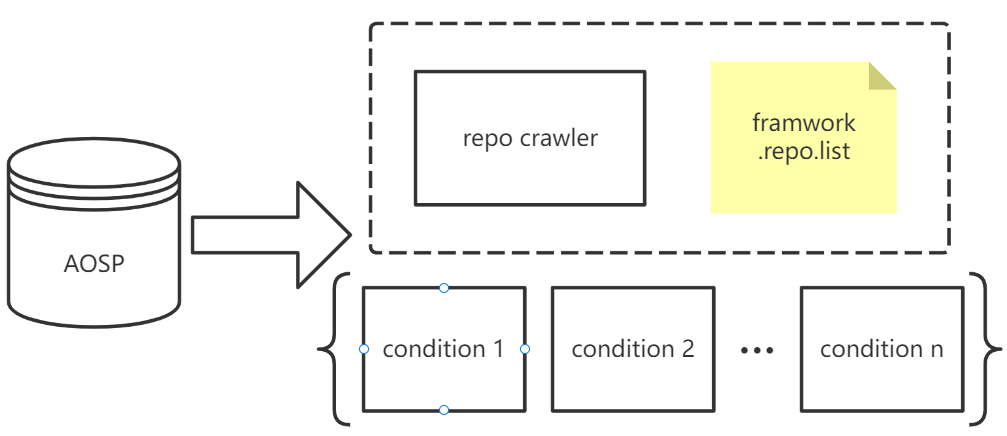
\includegraphics[width=.8\textwidth]{figures/archi-repo-crawler.png}
    \caption{repo\_crawler 设计图}
    \label{fig:archi-repo-crawler}
\end{figure}

\subsubsection{Android.bp 文件收集:bp\_collector}

soong 构建系统在运行之初会调用 Blueprint 模块。Blueprint 模块的主要执行过程大致可被分为三步:收集 Android.bp 文件,将 Android.bp 文件中的 Blueprint 语法转化为 ninja 语法,输出到 ninja manifest 文件中。soong 在运行时会输出一份从各个路径中寻找存在 Android.bp 的目录,并将该目录输出在 out/.module\_paths 下的 Android.bp.list 中。因此可以有效利用该文件收集散布于整个 AOSP 中的,且在构建过程中被使用到的 Android.bp 文件。该部分设计逻辑如图\ref{fig:archi-bp-collector}所示。

\begin{figure}
    \centering
    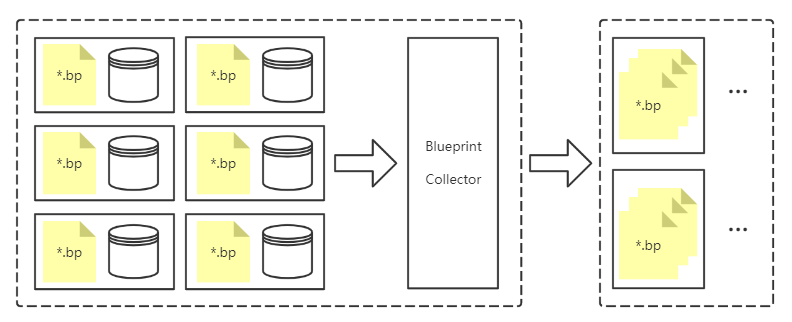
\includegraphics[width=.8\textwidth]{figures/archi-bp-collector.png}
    \caption{bp\_collector 示意图}
    \label{fig:archi-bp-collector}
\end{figure}

\subsubsection{仓库-模块关系:pkg\_repo\_tool}

根据第二步的结果,将收集到的所有 bp 文件放在一个路径下。利用 Blueprint 中的 parser 模块解析收集到的 bp 文件,使用 Go 语言编写应用程序,要求输入第一步中得到的仓库名,输出具体内部项目 / 模块 / 仓库三者之间的联系到一个 json 文件当中。该部分的架构图如图\ref{fig:archi-pkg-repo-tool}所示。

\begin{figure}
    \centering
    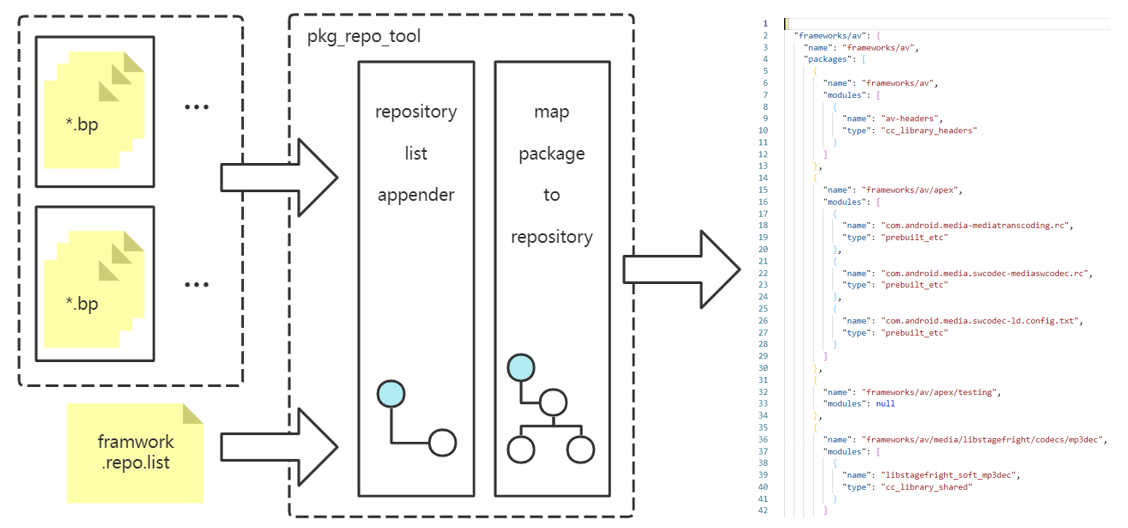
\includegraphics[width=.8\textwidth]{figures/archi-pkg-repo-tool.png}
    \caption{pkg\_repo\_tool 示意图}
    \label{fig:archi-pkg-repo-tool}
\end{figure}

\subsection{获取软件变更:diff\_extractor}

通过给定的仓库与两个版本的 commit id,可以利用 git 中的数据结构,获得两版本间存在差异的文件名。与此同时,本系统选用 GumTree 作为抽象语法树节点级别的变更获取工具,并使用算法\ref{alg:get-method-name},从 GumTree 给出的变更节点向上回溯至方法定义节点与类定义节点,进而获取两版本间存在差异的方法名与类名。该模块架构如图\ref{fig:archi-diff-extractor}所示。

对于 diff\_extractor 的具体实现而言,该模块使用了 eclipse.jgit 解析 git 仓库中的数据结构,并使用 GumTree 获得基于抽象语法树的细粒度软件变更。jgit 可以根据输入的信息,获得诸如变更文件名、具体变更文本以及变更前后的源代码等。该项目将变更前后的源代码传入 GumTree,再根据获得的输出基于抽象语法树节点标签判断,最终得到 json 格式的输出结果。

\begin{figure}
    \centering
    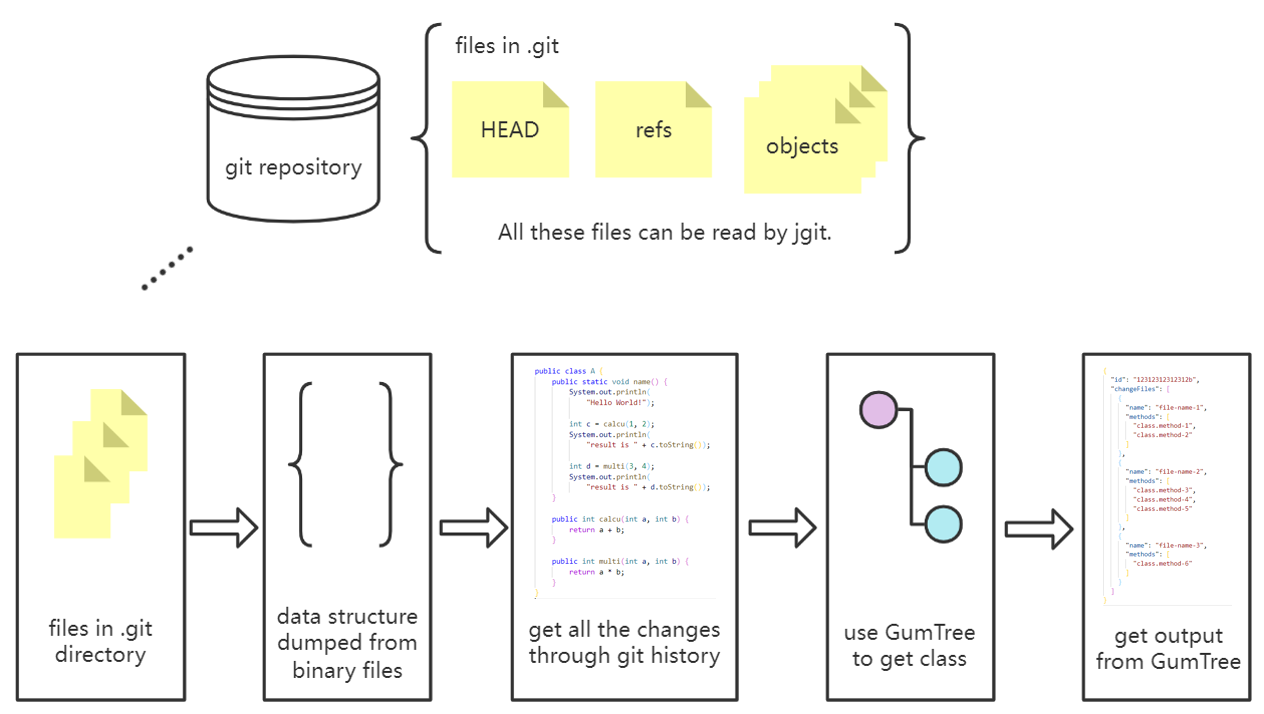
\includegraphics[width=.8\textwidth]{figures/archi-diff-extractor.png}
    \caption{diff\_extractor 示意图}
    \label{fig:archi-diff-extractor}
\end{figure}

\subsection{模块间分析功能}

\subsubsection{构建清单精简工具:manifest\_refinement}

在编译 AOSP 时,soong 构建系统中的 Blueprint 模块被自动调用生成 build.ninja 文件。然而,即便 ninja 语法相较于 Makefile 而言更为简单,用于描述 AOSP 完全构建过程的纯文本文件 build.ninja 仍需要占用 3 GB 左右的磁盘空间。对 ninja 文件进行分析依旧需要较大的资源。本系统为解决该问题,根据 Android.bp 文件所在路径使用文本匹配方法,剔除不在本系统考虑范畴之内(platform/frameworks)的构建过程。manifest 文件处理结果如图\ref{fig:archi-manifest-refinement}所示。

\begin{figure}
    \centering
    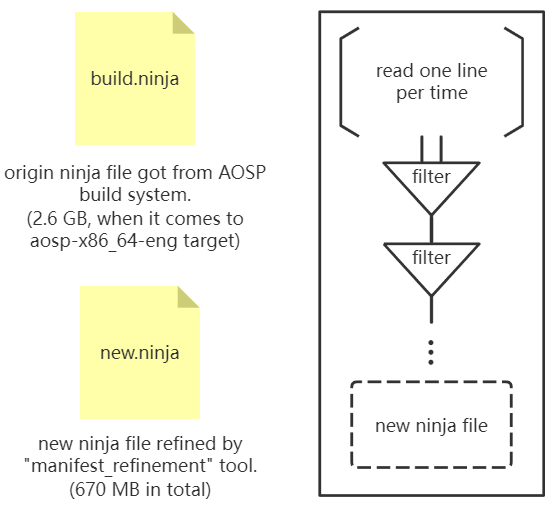
\includegraphics[width=.5\textwidth]{figures/archi-manifest-refinement.png}
    \caption{manifest\_refinement 示意图}
    \label{fig:archi-manifest-refinement}
\end{figure}

\subsubsection{求解扩展有向图中多源可达问题:ninja\_hacked}

Ninja 中使用 Node 抽象真实存在的文件,使用 Edge 抽象单一构建过程 “build”,进而利用 Node 与 Edge 数据结构构成有向无环图。在多源可达问题求解中,首先需要确定所有的存在变更的源文件。在 AOSP 的构建过程中,如果一个文件并非由 Ninja 构建系统中的构建过程给出,则说明该文件是源文件。也就是说,在 Ninja 所维护的有向无环图中,若一个 Node 仅有 in\_edge,而其 out\_edge 不存在或 out\_edge 并没有连接其余输出,则说明该 Node 对应的文件属于源文件。根据 AOSP 中 Ninja 的工作流程,存在变更的文件必定属于源文件。ninja\_hacked 项目的流程图如图\ref{fig:archi-ninja-hacked}所示。

Ninja 项目的本质是一个命令行工具,其中需要的参数都需要以命令行参数传入。Ninja 使用 ReadFlag 解析命令行参数 argv 到内部的 options 和 config 中。此后,Ninja 会进入执行构建任务的主循环中。对于主循环而言,一次循环即执行一次由一个 ninja 文件定义的完整构建过程。Ninja 中使用 ManifestParser 解析 ninja 语法,并使用其中的 Load 方法解析构建与规则,并将其全部实例化为 Edge 和 Node 对象。

ninja\_hacked 项目巧妙借助了 Ninja 中的 “插件功能”,即 Ninja Tool。在通过命令行使用 Ninja 时,可通过指定 “-t” 参数来决定 Ninja 的行为。在 Ninja 源代码中,这些行为包括但不限于 “基于一个构建目标获得其构建过程”、“根据已部分定义的目标生成构建依赖图” 等等。ninja\_hacked 利用 Ninja 的 Tool 编写规则,集成了名为 Origin 的 Tool,该工具可以根据给定的 manifest 文件以及给定的源文件,得到其所有可能影响的源文件、中间文件与最终产物,并将这些信息以 json 形式输出到文件中。

\begin{figure}
    \centering
    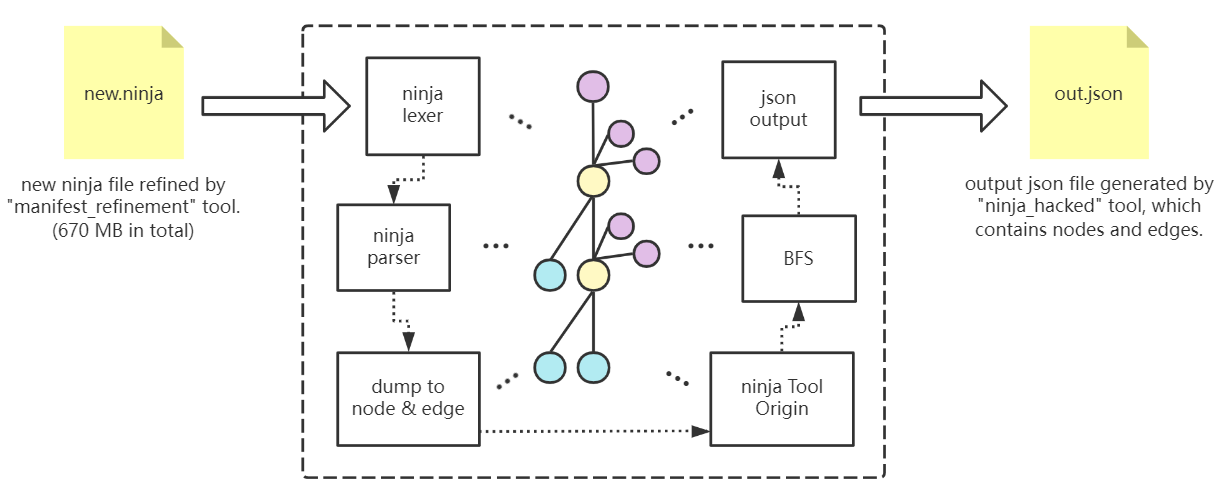
\includegraphics[width=.8\textwidth]{figures/archi-ninja-hacked.png}
    \caption{ninja\_hacked 示意图}
    \label{fig:archi-ninja-hacked}
\end{figure}

\subsubsection{文件间影响可视化:deps\_reflection}

为方便展现模块间分析中文件影响关系,本系统在进行模块间分析的同时输出影响关系文件。该文件可通过 deps\_reflection 项目转化为 Graphviz 工具的输入文件。deps\_reflection 项目内部模拟了 Graphviz 内的 Node 与 Edge 数据结构,使用 ninja\_hacked 项目的输出文件作为输入,将其中的文件视作节点,将文件与文件间的依赖关系视为边,使用传统有向图构建依赖关系图。输出结果如图\ref{fig:archi-deps-reflection}所示。

\begin{figure}
    \centering
    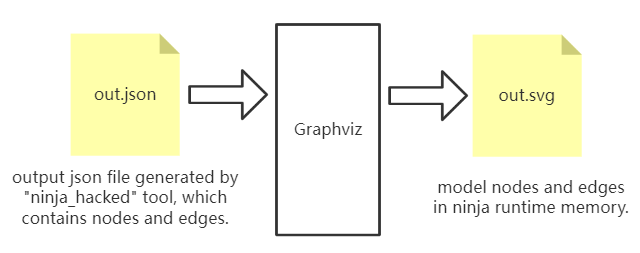
\includegraphics[width=.8\textwidth]{figures/archi-deps-reflection.png}
    \caption{deps\_reflection 示意图}
    \label{fig:archi-deps-reflection}
\end{figure}

\subsection{模块内分析:cg\_generator}

本系统使用调用图确定给定的变更方法对模块内其他方法造成的影响。AOSP platform/frameworks 的本质是一套有关 Android 应用开发的核心框架,用户可以通过继承等方式扩展 platform/frameworks 中定义的类。同时,platform/frameworks 中只有属于库的公共 API 的代码被库的用户扩展,所有只能通过不属于公共 API 的代码访问的代码都被认为属于库的实现。\cite{CALLGRAPHCONSTRUCTION}面向 AOSP 分析的初衷是获取两版本间软件变更对未合入主分支的代码的影响,仍旧是依托于用户应用进行的库分析,所以对库进行分析时需要关注的部分相对较少。

本系统中使用的调用图生成装置基于开源工具 Java Call Graph 开发,增加了对 AOSP 中构建产物的适配,完善了以方法调用指令为基础的访问者模式,可以根据变更方法的类名与方法名获取其影响的方法集合。该部分架构如图\ref{fig:archi-cg-generator}所示。

cg\_generator 模块需要传入真实存在的 jar 文件。在具体实现上,项目使用 util.jar 中的 JarFile 与 JarInfo 获得 jar 文件内各 class 文件入口以及 jar 文件元信息。对于每一个 class 文件,项目都使用一个独立的 apache.bcel 中的 ClassParser 解析字节码获得 JavaClass 类的实例化对象。针对每一个 JavaClass,项目中使用自定义的 ClassVisitor 进行独立分析。JavaClass 中存在本属于字节码文件内但已被解析的常量池、属性区以及方法区等概念。对于 JavaClass 对象内的每个方法,ClassParser 已将其实例化为一系列 Method 对象。而针对每一个 Method,项目中又使用自定义的 MethodVisitor 进行独立分析。每个 Method 中都存在一条由一系列类型不同但都继承于同一父类 Instruction 的子类组成的链表,因此 MethodVisitor 遍历当前方法下的所有 instruction,对每条 instruction 都进行判断,确定在生成方法调用图这一场景下是否需要将其纳入考虑范围内。

对于 Java 语言,Java 7 增加的 invokedynamic 指令是使用字节码文件分析调用图的问题之一,并且在 Java 8 中新增的 Lambda 函数底层便是使用该 JVM 指令执行。invokedynamic 指令原本有 4 个操作数,其中前两个操作数共同构成了查找常量池中 CONSTANT\_InvokeDynamic\_info 的索引,以便于查找 Bootstrap method 并将参数传入。对于每一条 invokedynamic 指令执行的位置,JVM 都将其视为一个动态调用点,cg\_generator 模块使用容器来存储调用点所在的方法以及调用的目标。

需要说明的是,由于 JavaClass 中成员与 Method 中成员大致相仿(JavaClass 下有 Method 列表,Method 下有 Instruction 链表),因此 ClassVisitor 与 MethodVisitor 的设计也十分相似。

\begin{figure}
    \centering
    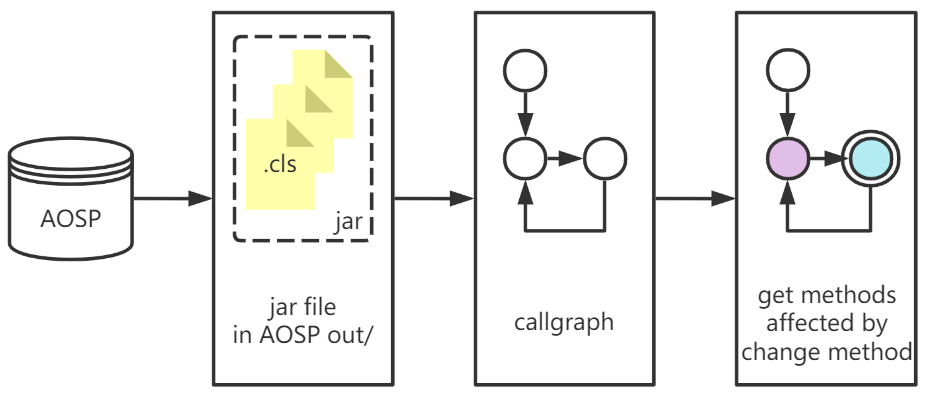
\includegraphics[width=.8\textwidth]{figures/archi-cg-generator.png}
    \caption{cg\_generator 示意图}
    \label{fig:archi-cg-generator}
\end{figure}

\subsection{模块实验结果}

\subsubsection{repo\_crawler 实验结果}

AOSP 中仓库分布并无规则,存在两同级目录属于不同仓库的情况(如 platfrom/frameworks/av 与 platform/framework/native),但同时也存在多级目录作为仓库被维护的情况(如 platform/framework/opt/bitmap 与 platform/framework/opt/car/services)。因此需要即时爬取并解析 googlesource 上的数据。 该系统利用 Python 的 requests 和 bs4 获取 platform/frameworks 下的 67 个仓库名称。该小型应用工具作为模块间分析流程的第一步,模块设计如图\ref{fig:design-repo-list}所示,具体实现可见 \href{https://github.com/AOSPworking/repo_crawler}{repo\_crawler}。

\begin{figure}
    \centering
    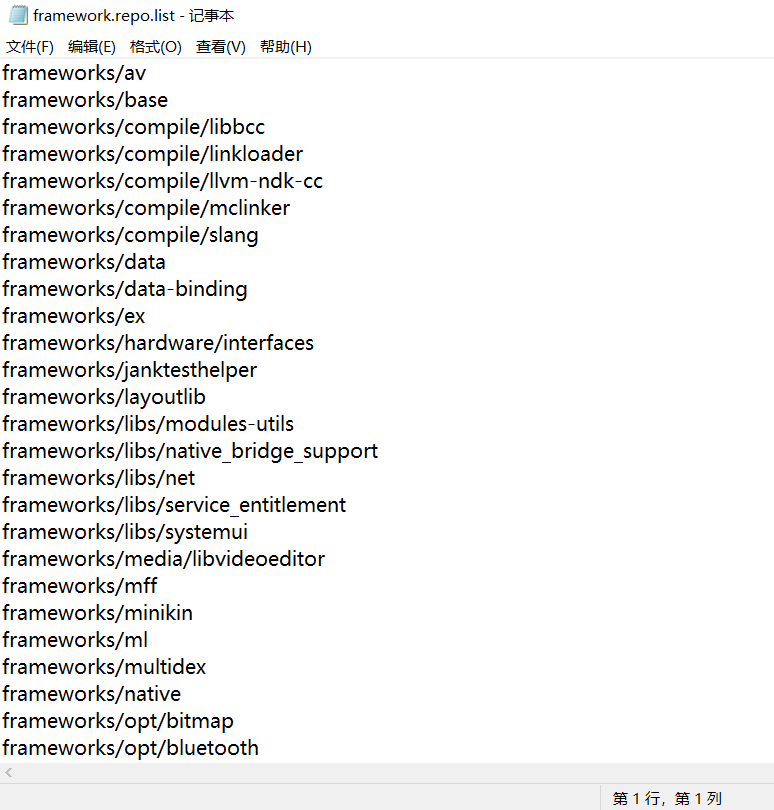
\includegraphics[width=.4\textwidth]{figures/design-repo-list.png}
    \caption{爬取 frameworks 下所属仓库获得的名称列表}
    \label{fig:design-repo-list}
\end{figure}

\subsubsection{pkg\_repo\_tool 实验结果}

仿照 soong 构建系统在运行初调用 Blueprint 模块的行为。bp\_collector 旨在获取给定路径下的所有 Android.bp 文件。bp\_collector 选择借助 soong 构建系统运行时输出的 Android.bp.list 文件,该文件是 soong 运行时收集各路径下 Android.bp 文件的依据,存储在 out/.module\_paths 下。bp\_collector 正是依靠该文件的生成逻辑,从 AOSP 中各目录中获取文件,并存储在指定的文件夹下,以方便后续分析。

由于 AOSP 下的 Blueprint 项目是一个较为独立的项目,相较于 soong 这一必须基于 AOSP 目录结构才能运行的系统,Blueprint 更像是为 soong 提供有关 bp 文件操作能力的插件。根据 bp\_collector 的执行结果,pkg\_repo\_tool 模块内部利用 Blueprint 中的 parser 模块解析收集到的 bp 文件,获得仓库到模块的关系如图\ref{fig:design-repo-pkg-relation}所示,该模块具体实现可见 \href{https://github.com/AOSPworking/pkg_repo_tool}{pkg\_repo\_tool}。

\begin{figure}
    \centering
    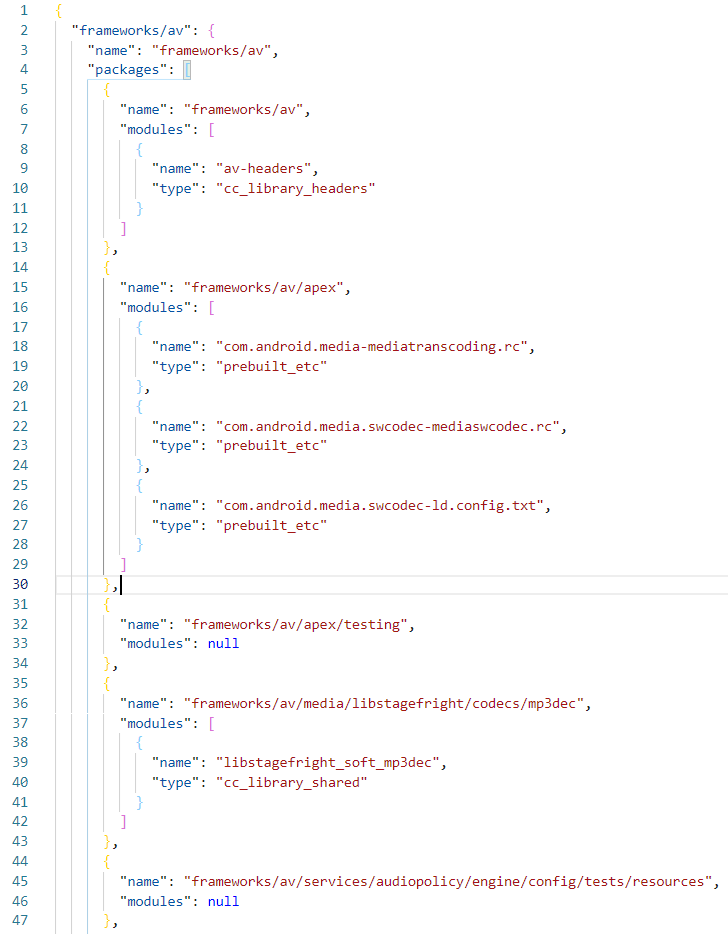
\includegraphics[width=.4\textwidth]{figures/design-repo-pkg-relation.png}
    \caption{解析得到 AOSP 下各仓库内模块情况}
    \label{fig:design-repo-pkg-relation}
\end{figure}

\subsubsection{diff\_extractor 实验结果}

通过输入给定仓库所在路径与两个版本的 commit id,借助 .git 目录下 的数据结构,获得通过 jgit 库效仿 git diff 指令获得两版本间差异(在 jgit 中,用于描述差异的类被称作 DiffEntry,通过 DiffEntry 可以获得存在差异的文件名以及具体文本差异)。本系统选用 GumTree 作为抽象语法树节点级别的变更获取工具。通过 DiffEntry 中获得的文件名以及输入的 commit id,可从 .git 中的对象文件中获取对应 commit id 下指定路径文件内容。使用算法\ref{alg:get-method-name},可从 GumTree 给出的变更节点向上回溯至方法定义节点与类定义节点。结果如图\ref{fig:design-diff-extractor}所示,该模块具体实现可见 \href{https://github.com/AOSPworking/diff_extractor}{diff\_extractor}。

\begin{figure}
    \centering
    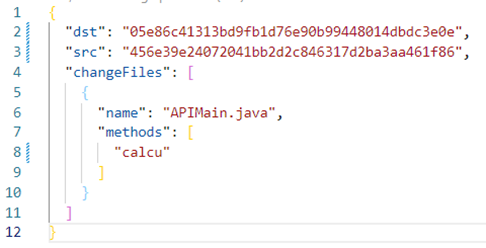
\includegraphics[width=.4\textwidth]{figures/design-diff-extract.png}
    \caption{扫描 AOSP 编译产物获得存在变更的类以及方法的元数据信息}
    \label{fig:design-diff-extractor}
\end{figure}

\subsubsection{manifest\_refinement 实验结果}

用于描述 AOSP 完全构建过程的纯文本文件 build.ninja 仍需要占用 3 GB 左右的磁盘空间,在使用 manifest\_refinement 项目对 build.ninja 文件按条件过滤后,得到的 new-build.ninja 仅有 670 MB 左右。由于扩展有向图的复杂程度与 $O(F + B)$ 有关,而 build.ninja 中的文件中大多数篇幅在定义扩展有向边,因此对 build.ninja 文件的精简可以有效缩减对 ninja\_hacked 项目进行分析时需要的资源。manifest 文件处理结果如图\ref{fig:archi-manifest-refinement}所示,该模块具体实现可见 \href{https://github.com/AOSPworking/manifest_refinement}{manifest\_refinement}。

\begin{figure}
    \centering
    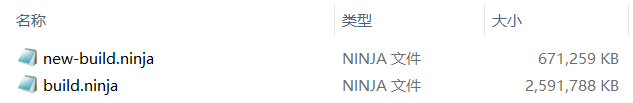
\includegraphics[width=.8\textwidth]{figures/design-manifest.png}
    \caption{AOSP 构建过程描述文件 build.ninja 处理结果}
    \label{fig:design-manifest}
\end{figure}

\subsubsection{ninja\_hacked 实验结果}

相较于插桩、获取运行时内存的手段,借助 Ninja 中的 Node 与 Edge,充分重用已有数据结构编写程序,并将其集成到原有项目中的方法更加具有操作性。Ninja 中使用 Node 抽象真实存在的文件,使用 Edge 抽象单一构建过程,利用 diff\_extractor 模块的输出作为本模块的输入,获得两版本间存在代码变更的文件名。在 Ninja 所维护的有向无环图中,源代码文件对应的 Node 仅有 in\_edge,而其 out\_edge 不存在或 out\_edge 并没有连接其余输出。进而可以使用广度优先搜索算法,得到的因变动而被影响的文件列表,结果如图\ref{fig:design-node}所示。

在此基础上,运用算法\ref{alg:intermodule-analysis}可以得到 AOSP 构建中所有因给定变更文件集合而受到直接或间接影响的文件集合。描述此类影响关系的内容如图\ref{fig:design-edge}所示。该模块具体实现可见 \href{https://github.com/AOSPworking/ninja-hacked}{ninja\_hacked}。

\begin{figure}
    \centering
    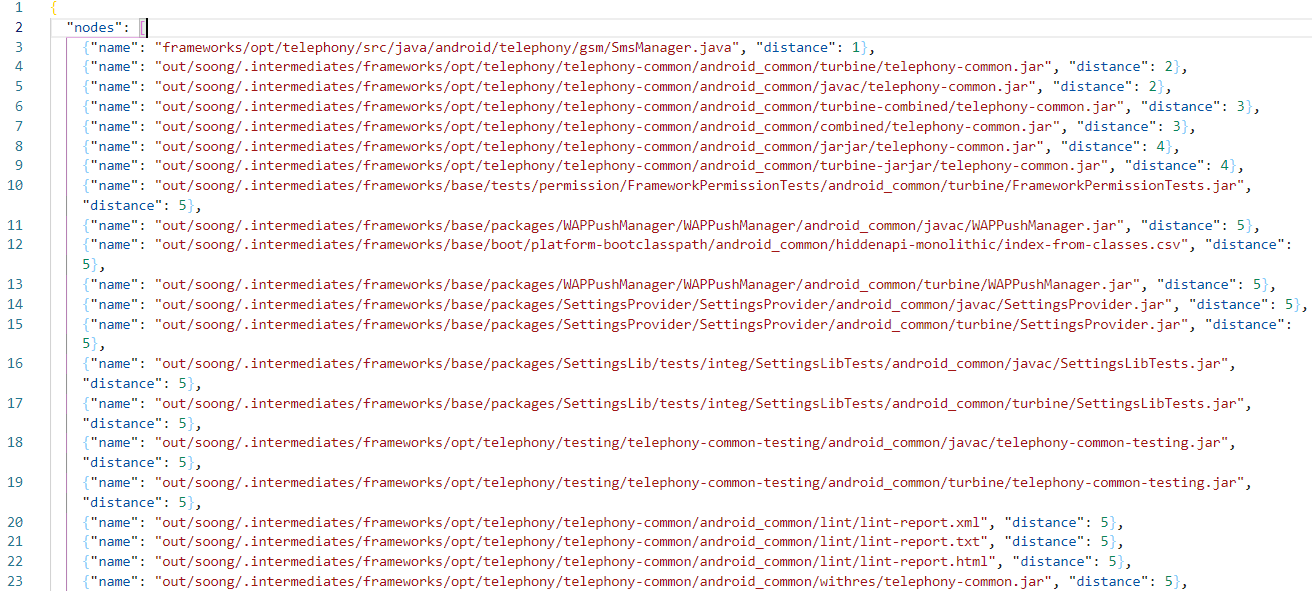
\includegraphics[width=.8\textwidth]{figures/design-node.png}
    \caption{基于给定变更而遭到影响的文件列表}
    \label{fig:design-node}
\end{figure}

\begin{figure}
    \centering
    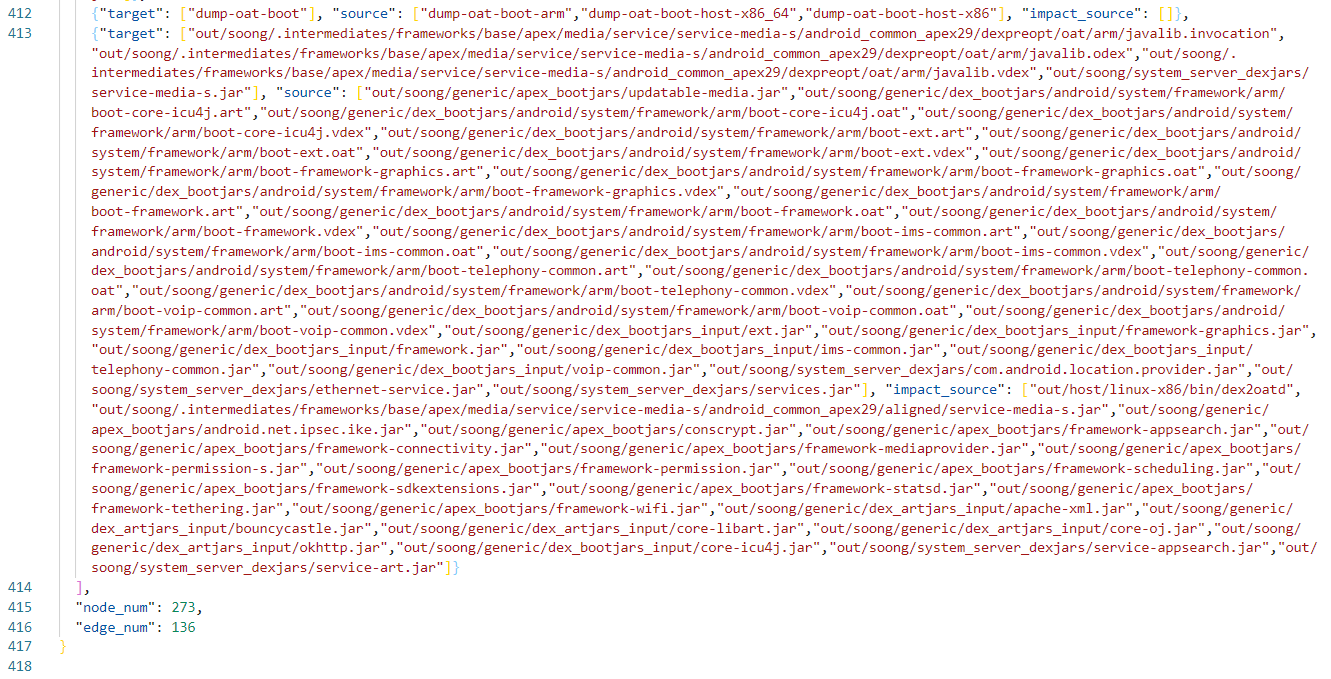
\includegraphics[width=.8\textwidth]{figures/design-edge.png}
    \caption{ninja\_hacked 输出文件中描述的文件间影响关系}
    \label{fig:design-edge}
\end{figure}

\subsubsection{deps\_reflection 实验结果}

deps\_reflection 使用 Graphviz 展现模块间分析中文件影响关系。本模块使用了 ninja\_hacked 模块输出的 json 文件,使用 JavaScript Graphviz 库中定义的 node 与 edge 类模拟 json 中定义的对象,使用传统的有向图构建依赖关系图。由于 AOSP 体积过于庞大,构建过程过于复杂,以至于一个源文件能够直接影响的中间产物与目标产物以及构建过程就有上百个。因此为可视化更为美观,deps\_reflection 屏蔽了间接影响的文件。由于本模块仅仅用于可视化,并不修改 ninja\_hacked 的输出文件,因此屏蔽间接影响文件是可行的。该模块输出结果如图\ref{fig:design-deps-reflection}所示,具体实现可见 \href{https://github.com/AOSPworking/deps_reflection}{deps\_reflection}。

\begin{figure}
    \centering
    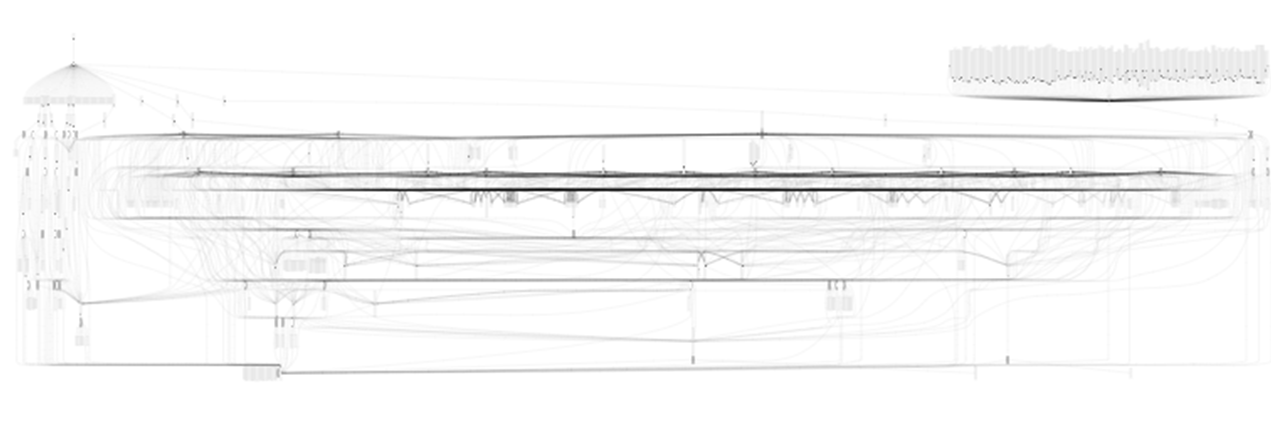
\includegraphics[width=.8\textwidth]{figures/design-view.png}
    \caption{deps\_reflection 构建的依赖关系图}
    \label{fig:design-deps-reflection}
\end{figure}

\subsubsection{cg\_generator 实验结果}

cg\_generator 中所使用的调用图构建方法基于 Java Call Graph 开发。Java Call Graph 使用访问者模式这一时常出现在各类静态程序分析框架中的设计模式开发。我在原本的 Java Call Graph 基础上,拆分了对 method 与 instruction 的访问方式,我所作出的改进大幅度改善了项目代码的可读性和可扩展性,可以针对 method 与 instruction 明确地进行不同的分析。具体而言,项目使用了 Apache BCEL 字节码操作库,确定给定的变更方法以及方法内的方法调用状况。在为所涉及的方法创建节点(包括实际节点与虚拟节点)的同时,构建方法与方法间的调用关系图,即对模块内其他方法造成的影响。完善的以方法调用指令为基础的访问者模式,可以根据变更方法的类名与方法名获取其影响的方法集合。除此之外,我增加了对 AOSP 结构与其中构建产物的适配(如 AOSP 构建过程得到的 jar 包中的部分 class 文件可能存在无代码区的问题)。所得结果如图\ref{fig:design-cg-generator}所示,该模块具体实现可见 \href{https://github.com/AOSPworking/cg_generator}{cg\_generator}。

\begin{figure}
    \centering
    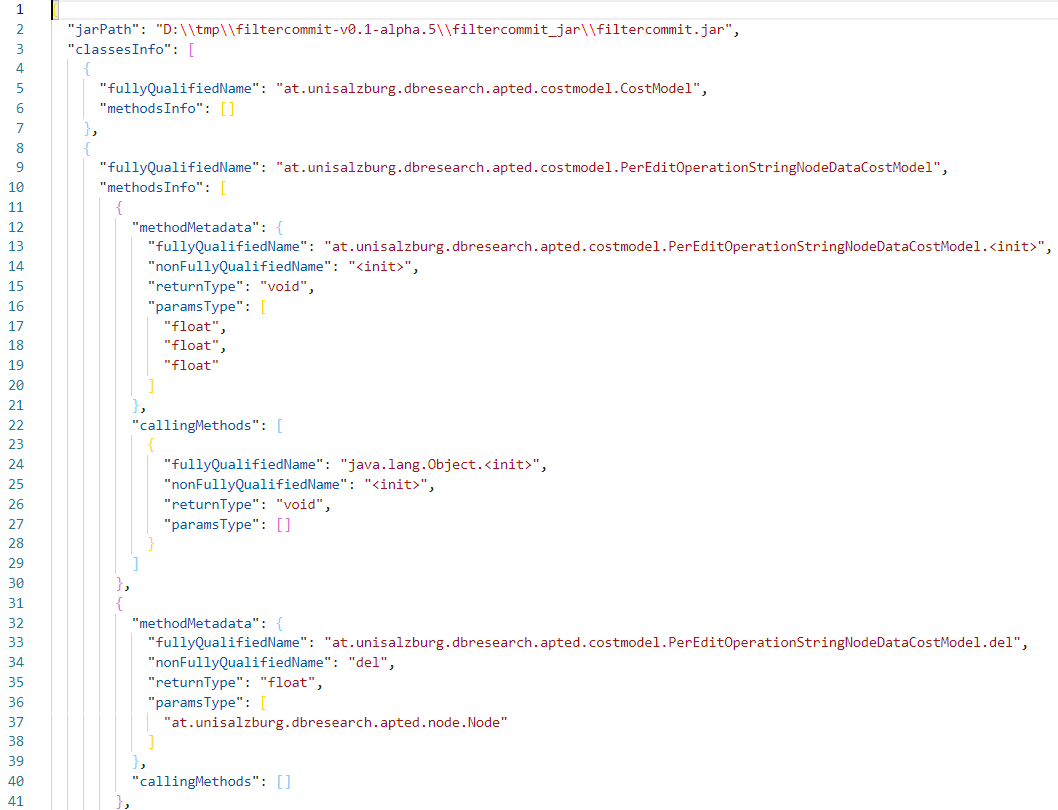
\includegraphics[width=.6\textwidth]{figures/design-cg-generator.png}
    \caption{方法调用图中保存的元数据信息}
    \label{fig:design-cg-generator}
\end{figure}

综上所述,本文所设计的软件变更分析系统在 AOSP 场景下重点体现在 “依照构建系统完成数据处理”、“变更获取”、“模块间分析” 以及 “模块内分析” 三点。本系统以 AOSP 下的 platform/frameworks 为例,在数据预处理方面获得其下的 67 个仓库,并与 5804 个模块建立了联系;在变更获取方面,根据给定的仓库路径和 commit id,能够成功做到获取存在变更的方法以及所属类;在模块间分析方面,成功将 2.7GB 的 build.ninja 文件精简为 670MB,大幅缩小了分析范围,且能够根据给定源文件使用 Ninja 内部数据结构导出全部影响关系;在模块内分析方面,能够根据给定的 jar 文件得到调用图,并根据输入的方法名得到所有与该方法相关的方法列表。
\newpage
\section{总结}\label{summary}

光阴似箭。自 2021 年 10 月初毕业实训与毕业设计题目上报开始,到 2022 年 5 月毕业设计论文的撰写结束,将近 7 个月的毕业设计即将落下帷幕了。毕业设计作为本科学习生涯中最后一道关卡和最重要的一项设计任务,同时也象征着本科阶段的总结与新阶段的开启。在此次毕业设计中,我自认无愧于大学本科四年来所获得的理论知识与实践本领,本次毕业设计项目算是我交给过往四年的一份较为满意的答卷。对此,我进行了如下总结。

\subsection{毕业设计总体执行情况}

毕业设计作为本科四年学习过程的最后一个任务,不仅需要综合考察所学专业知识与技能本领,还需要作为总结过往、开启未来新阶段的一项工作。作为同济大学电子与信息工程学院计算机科学与技术系的一名学生,我能够感受到学院各级领导对本科生毕业设计任务的重视程度——去年下半年的毕业实训与毕业设计动员会令我对毕业设计的重要性有了极其明确的认识。这也使得我在上学期末认真地撰写了毕业实训报告,并对本学期的毕业设计任务进行展望。

我在本次毕业设计过程中接触了先前从未接触过的计算机科学领域中的一个方向,在导师的指导下从无到有地建立了理论基础、获得了实践经验。

在这过程中,我首先接触了 AOSP 的构建系统,阅读了 soong 构建系统中 soong-ui、Blueprint 等模块以及 Ninja 构建系统的大部分源码,共计 30000 余行。我通过该阶段对 Ninja 构建步骤以及 Ninja 内部各关键数据结构有了一定的掌握,这为我后续在代码规模 1 万余行的 Ninja 上继续开发新功能做了铺垫。

此后,我学习并阅读了 Ninja 用于描述构建过程的清单文件。现代移动端操作系统无论在源代码还是最终的构建产物都是一个庞大的巨无霸,以至于用于描述其构建过程的文本文件就有 2.7 GB 左右的大小。阅读并从该文件中提取有效信息是整个毕业设计中最为困难、最为耗神的步骤。在该阶段,我将 build.ninja 文件、soong Blueprint 模块源代码以及 Ninja 构建系统源代码结合起来阅读,这使得我成功总结出 build.ninja 中的特殊文件格式,令我后续的开发得以顺利进行。

紧接着,我学习了多种变更相关工具的理念和使用。我较为深入的了解了现今 git diff 所使用的算法,学习了 gumTree 与 CLDIFF 的使用。优雅地设计变更获取模块并不是一件简单的事,我曾纠结于使用 jdt AST 还是 gumTree 提供的结构,也曾纠结于 CLDIFF 在算法实现方面提供的简便与其他开源库的便捷。最后我仍屈服于 gumTree 的便捷,使得我的程序略显丑陋。

最后,我学习了多种开源调用图生成工具的使用。无论是 Soot、WALA 还是 Java Call Graph,都存在文档落后、不适配现有场景的问题。解决该问题是一条漫长的道路,我从零开始,从 JVM 类加载过程开始学习,从类文件结构开始学习,一点一点地发现、归纳、搜索、学习并解决面前的问题,这才有了 cg\_generator 简短的 1000 余行代码。

本次毕业设计选题与实际应用具有较紧密联系,时间较长,内容较为充实——我阅读了近 30 篇文献,阅读了 30000 余行代码,上文中所设计的系统涉及 8 个代码仓库,并使用了 7 种不同的通用编程语言开发,仓库内代码总计 7000 余行,能够完成任务书中描述的功能。毕业设计总体执行情况较为顺利。

\begin{itemize}
    \item 从本学期第 1 周开始,我以上学期的毕业实训中所做理论铺垫为基础,深入阅读了 soong 构建系统中 Blueprint 部分与 bootstrap 部分的源代码(10k LoC)、Ninja 中有关构建过程与插件功能的源代码(10k LoC),证明了模块间变更分析模块实现的可行性。
    \item 第 2 周到第 4 周,我基于第 1 周所学习到的理论,为 Ninja 构建系统增加特性,并对毕业实训中设计的工具进行修改。
    \item 第 5 周到第 6 周,我通过阅读相关文献以及学习 jgit 与 jdt 的使用,获得变更差异具体到源文件的影响。
    \item 第 7 周到第 11 周,我学习了各种开源程序分析框架的用法,学习了 JVM 字节码操作库 Apache BCEL,并修改 Java Call Graph 令其能够使用 AOSP 中的 jar 文件生成调用图。与此同时,我完成了论文翻译工作。
    \item 第 12 周及以后,我逐步撰写毕业论文。
\end{itemize}

\subsection{毕业设计中遇到的困难}

在毕业设计过程中,我确实遇到了诸多方面的困难,其中甚至有部分难题令我一度以为毕业设计不存在实际可行性,也有部分困难在毕业设计中没有得到解决。

\subsubsection{相关资料的匮乏}

本次毕业设计以 AOSP 为背景,然而中文互联网中与 Android 相关的资料大部分与 Android 开发有关,而与 AOSP 体系结构、构建系统相关资料较为匮乏。另一方面,Android 生态较为活跃,网络上可获取的资料大部分也不具备时效性(例如,我曾浏览过有关 Android.mk 书写规范的博客,但 Android Marshmallow 后逐渐使用 Android.bp 代替前者)。

\subsubsection{开源工具难以直接处理实际问题}

在计划生成调用图时,我调研过部分开源程序分析框架。但与 AOSP 类似的,这些框架作为实验室产品(非商业级应用)也具有缺乏文档说明、缺乏开发团队维护的缺陷。由于我本人理论基础与实践经验的不足,在框架的应用理解上也缺乏触类旁通、举一反三的快速学习能力。因此,存在相当长的一段时间,我认为通过开源工具生成调用图还不如自己实现。

\subsubsection{外界环境因素的干扰}

2022 年 4 月 3 日,嘉定校区正式开始封闭式管理。也许是我个人意志不坚定的缘故,长期封闭式管理确实对我的作息以及生活安排造成了一定影响。

\subsection{毕业设计感想}

本次毕业设计使我回忆起了学习的感觉。我非常高兴的是,在此次过程中,我接触了一个之前没有了解过的新领域,我也因此久违地体验到了学习的痛苦与乐趣。此前近两年时间,我都在舒适的浅水区中游泳,等到这次毕业设计的海浪拍向我,我才回忆起刚进入大学时、刚接触本专业的学习时、刚敲下第一行代码时的那份谨慎小心。

本次毕业设计使我认可了自己的学习经历。由于本课题是在我刚刚确认导师后不久得到的,因此我最初对其并无任何了解。在我逐渐了解课题后,令我感到惊讶的是,该课题看似是一项工程任务,但涉及的核心算法却涉及到数据结构与离散数学课程中学习到的知识。例如,在阅读 Ninja 源代码时,我能够直接看出其中各个工具使用的算法。这令我非常激动。

但同时,我必须承认本次毕业设计暴露出了我专业能力不足的问题。我本人在工程能力上仍有较大的缺陷——开发某模块后,不出两周就需要重新理解,这说明我个人的代码规范以及对项目的掌控能力不足。同时,在开发中我两次遭遇到已完成的模块间不能联通的情况,这说明我对项目的标准控制不足。我还有很长一段路要走。

在本科的最后一学期中,我通过该课题不断学习的过程中不断丰富理论知识,在不断开发的过程中不断提高实践本领。在老师的指导下一步步从开题报告、中期报告走到毕业论文这一关。本次毕业设计是对我个人四年以来所学专业技能的一个巩固与考察,让我理解了本科阶段所学知识的重要性,也提醒了我作为一名计算机专业学生需要持之以恒、积极进取、“终身学习”。

\subsection{对该工作未来的展望}

AOSP 作为 Google 主导维护的 Android 系统开源项目集合,是各大移动设备厂商关注的焦点。AOSP 庞大的体系架构中包含难以预估的复杂性,无论是对软件工程理论在实践中的应用,还是自动化、智能化工具在研发流程上的使用,都是一种巨大的考验。本文所设计的系统仅是围绕 AOSP 构建系统展开的应用开发,而 AOSP 还有许多主题或特性会为研发流程带来负担,如对新增代码的代码复杂度确定、基于目标仓库变更的文档生成、对合码过程中自研代码对 AOSP 各仓库的依赖面确定等。

\newpage

\addcontentsline{toc}{section}{参考文献}
\bibliography{note}

\newpage
\section*{谢辞}
\addcontentsline{toc}{section}{谢辞}

四年过去了。

其实没有特别大的变化。

2018 年 9 月 5 日上午,我和我爸妈站在校门口那个写着 “同济欢迎你” 的巨大展板前。那时的我绝对想不到四年过后的现在是怎样的。我眼中的世界在变化,我所处的社会在变化,我所在的学校在变化,我的家庭在变化,我的朋友们在变化,我也因此而变化。尽管一切都在不断地变化,我却还要说 “其实没有特别大的变化”。纷繁复杂花哨绚丽的事带不走我的一切,还不如迎面吹过的风。只不过,现在我正使用着我小学三年级就都认得的文字,写着我以往任一时刻都无法拼接出的词句段落。

毕业设计论文的致谢部分本不应如此沉重,但在这个时代背景下,我很难不用深沉的话语叙述我的过往、现在以及未来——过去四年里我通过各种途径学到了一些知识,这个过程十分曲折,我误入了很多不必要的陷阱。但我一直要求自己动用一切手段记住那些令我怄气、懊悔、愤恨、恼怒的事来提高我的精神耐受力,以便我未来再次遭遇它们时能做出更冷静的判断和更正确的解答。昨日种种,皆成今我,我做不到与过去的一切断绝联系。但与此同时,我正站在人生中某一阶段的最后关头,我想我还是有理由在此向我眼中的世界致谢。

在这不算成功的四年里,我受到了来自各方面的鼓励与支持。在这里,我首先要感谢我的家人们——感谢我的奶奶、我的爸爸以及我的爷爷。从小学到现在,我的家庭情况一直非常不好,这里需要尤其感谢奶奶对我的付出。虽说现在大学扩招严重,本科学历占总人口比例急剧攀升,但高考考上我校并写完毕业设计也算不辜负我奶奶对我的期望了。

接下来,我想感谢在这四年里提供给我帮助的老师们。这里我要感谢沈坚老师、陈宇飞老师、郭玉臣老师、卫志华老师、邓蓉老师。(以所学课程时间为序)感谢各位老师在课上课下对我的照顾。这里还要感谢我的研究生导师董震老师,其实拿到这个题目后,我一度以为自己无法完成,也有相当长的一段时间心情非常忧郁。好在老师给我提供了极为有效的指导,让我能够在正确的道路下不断前进。

此后,我想感谢现代大学制度。对我而言,大学最值得赞美的,莫过于它提供了一个结识同龄人的平台。感谢同济大学,你为我们提供了一个共同的话题。

因此,最后也是最重要的,我想感谢大学四年来为我提供了各方面帮助的各位同学!

首先我想感谢的是到了大学还与我有密切联系的高中同学们。这里我要感谢中央财经大学的雷诗雨同学、中国人民大学的饶迪同学、我校的孙汇通同学、大连理工大学的吴昊楠同学、北京大学的余舟{\CJKfontspec{宋体}飏}同学、重庆大学的张辰星同学、北京理工大学的周亮同学以及北京大学的周星宇同学。(以姓名拼音为序)感谢以上同学对我精神上的支持与帮助,感谢你们的理解与包容。

我还要感谢在本科四年中确实改变了我人生轨迹的同学们。这里我要着重感谢 17 级自动化专业的王怡琳同学、本专业的李培昊同学与吴子豪同学、17 级计科专业的刘佳伟同学、18 级计科专业的鞠璇同学与赵中楷同学、16 级计科专业的颜正辉同学以及我校软件学院 18 级的刘雪迪同学。(以影响我的时间前后为序)与从真实世界获得的感悟相比,这四年里我在课堂与书本上得到的知识极为有限。我十分感激在我校遇到了许多能改变我自己的人。

接下来,我要感谢我的室友们,感谢 18 级计科专业的郭嘉胥同学、纪宇同学、李宇龙同学、杨宏辉同学以及 18 级信安专业的甘源同学、胡新邦同学、许帅同学。(以时间与姓名拼音为序)室友是我本科四年里陪伴我时间最久的人,在这里非常感谢各位室友对我的照顾。

最后我想感谢这四年来同济大学里每一个和我展开过一定强度的线上闲聊的同学。再次感谢上面提到的王怡琳同学、李培昊同学、刘雪迪同学,感谢 18 级计科专业的俞少作同学、胡行健同学、张海同学、朱姝{\CJKfontspec{宋体}玥}同学、张晨阳同学,感谢 18 级自动化专业的陈旭海同学,感谢 18 级大数据专业的段抒彤同学、卞逸凡同学,感谢 19 级计科专业的周珂帆同学、彭斐然同学,感谢 19 级信安专业的商睿同学。(受篇幅限制,还望未被提及的同学不要介意)感谢这些同学在我孤独寂寞时与我聊天,愿过去的美好在过去永远美好。

本科四年过去了。我的毕业没有合照,没有聚餐,没有旅行。我拥有的只是一次匆忙的离去——而我带不走无奈散落在我桌前的许多回忆,以及一次又一次唐突的离别——而我事先并未知晓它们都是最后一次相见。我眼中的世界正遭受着莫大的考验,而我对此无能为力。

受制于篇幅,我很难在短短的一个章节内完全表露我此刻心中的所有感激之情。

感谢各位,祝这世界中的我毕业快乐。


\end{document}
